% Created 2024-01-19 Fri 09:41
% Intended LaTeX compiler: pdflatex
\documentclass[11pt]{article}
\usepackage[utf8]{inputenc}
\usepackage[T1]{fontenc}
\usepackage{graphicx}
\usepackage{longtable}
\usepackage{wrapfig}
\usepackage{rotating}
\usepackage[normalem]{ulem}
\usepackage{amsmath}
\usepackage{amssymb}
\usepackage{capt-of}
\usepackage{hyperref}
\author{Phil}
\date{\today}
\title{}
\hypersetup{
 pdfauthor={Phil},
 pdftitle={},
 pdfkeywords={},
 pdfsubject={},
 pdfcreator={Emacs 29.1 (Org mode 9.6.6)}, 
 pdflang={English}}
\begin{document}

\tableofcontents

\section{Introduction}
\label{sec:org02392f9}

\texttt{cl-naive-store} is a log structured document store. Documents are
loaded in-memory to facilitate fast querying. Depending on how you use
the store documents will be lazy loaded and indexed. It is written
completely in Common Lisp.

The "naive" comes from the fact that data is persisted
as plists in files to make them human and machine readable, also there
is no rocket science code.

The store was designed to be customisable, just about anything can be
customised, have a look at the implementation API to get an idea of
what is possible.

\subsection{Layered Design}
\label{sec:orgd392736}

\texttt{cl-naive-store} can do a lot but you as the user must decide how much
of the store's functionality you want to use for your own project.

Functionality was broken down into these packages:

\begin{itemize}
\item \texttt{cl-naive-store.naive-core}
\item \texttt{cl-naive-store.document-types}
\item \texttt{cl-naive-store.naive-documents}
\item \texttt{cl-naive-store.naive-indexed}
\item \texttt{cl-naive-store.tests}
\end{itemize}

The following .asd files can be used to load different functionality:

\begin{itemize}
\item \texttt{cl-naive-store.naive-core.asd} loads the most basic functionality for
\texttt{cl-naive-store}. Use this if you don't any of the other extensions.

\item \texttt{cl-naive-store.naive-merkle.asd} loads \texttt{naive-documents} and the
\emph{experimental} merkle functionality.

\item \texttt{cl-naive-store.naive-indexed.asd} loads \texttt{naive-core} and index
functionality.

\item \texttt{cl-naive-store.document-types.asd} loads \texttt{naive-core} and document-type
functionality.

\item \texttt{cl-naive-store.document-defs.asd} loads \texttt{naive-core}, document-types
and type definition functionality.

\item \texttt{cl-naive-store.documents.asd} loads naive-core, naive-indexed,
documents-types, definitions and document functionality.

\item \texttt{cl-naive-store.asd} loads the whole shebang.
\end{itemize}
\section{Releases}
\label{sec:org841eb11}

\subsection{Version 2023.12.19}
\label{sec:org8efcff7}

\subsubsection{Multiverse}
\label{sec:org2c0670f}

Added the concept of a multiverse to the store. The main reason was so
you can set up more complex data schemas with references across
stores.

\subsubsection{Code Refactor}
\label{sec:org9b24160}

There use to be a lot of different methods to add, remove and persist
stuff in naive store. This has been cleaned up to have just a couple
of methods like add-multiverse-element. Have a look at the
deprecation.lisp files for each layer for the details of what has been
deprecated. We use cl-naive-deprecation to ease the transition, your
code should run without you having to change anything
immediately. Eventually you will have to update your code.

In general the code is cleaner and the interface simpler to learn.

\subsubsection{Speed}
\label{sec:orge74f081}

Did work on cleaning up speed bottle necks.

\subsubsection{Bugs}
\label{sec:org7606eb9}

Many bugs where fixed during the conversion of the tests to cl-naive-tests.

\subsubsection{Tests}
\label{sec:orgb26f6f9}

cl-naive-store now uses cl-naive-tests and the tests where rewritten
for better coverage and to be cleaner.

You will learn a lot from reading the test code.

\href{home.org}{Home} :noexport: \href{home.org}{Previous} :noexport: \href{overview.org}{Next} :noexport:
\section{Overview}
\label{sec:orgd5c7db8}

\subsection{Log Structured Database}
\label{sec:org21e24d5}

At its core \texttt{cl-naive-store} is a log structured database.

A log-structured database is a type of database management system that
organizes and stores its data in a sequential, append-only
manner. Instead of overwriting data, it records all changes
as a continuous stream of log entries. Each entry typically captures
an operation, such as an insertion, update, or deletion, along with
the associated data.

Advantages of a log-structured database include:

High Write Throughput: Since all changes are simply appended, the
system can achieve high write speeds.

Simplified Crash Recovery: By replaying the log from a known good
state, the database can recover its state after a crash. The replaying
of the log however kicks you in the teeth when you get to tens of
millions of records.

Consistent Snapshots: By marking points in the log, consistent
snapshots of the database can be obtained without halting writes.

A log structured database can be slow to query if you query the files
directly. To overcome that \texttt{cl-naive-store} was designed to be an in
memory store. That means that when querying the data the file
structure does not come into play.

\texttt{cl-naive-store} has several layers of functionality that extends the
basic log store to a full document store. Each layer adds additional
functionality at the cost of increased overhead and complexity.

The concept of a document is only loosely implemented and enforced in
the base and indexed layers. It is when you use the full document
layer that the store becomes a proper document store.

\texttt{cl-naive-store} does not enforce the use of data schemas for your
data. Data schemas are optional and when used is only there to use as
a guideline, no strict enforcement of data schemas are done. This in
line with what is expected of a document store.

\subsection{Choosing Layers of Functionality}
\label{sec:org6c1e1fe}

Depending on the your use case you need to choose the appropriate
layer(s) to use. It must be noted that you can use a mixture of layers
depending on your requirements, this adds complexity to your data
schemas and will take a lot of testing to get the right balance.

As a rule of thumb using the full document layer will serve most
purposes well.

\subsubsection{Base Layer (Simple Log Database)}
\label{sec:orgc97c47c}

The base layer \texttt{naive-core} implements the basics of a log store with
in memory querying.

This layer has the smallest memory footprint per document and is the
least prescriptive as far as the structure of the data you use.

When should you use just the base layer?

\begin{enumerate}
\item Small Database

A couple hundred/thousand documents per collection. For example a
database serving a simple website.

\item Large Database with no keys

An example would be an event logger or such.
\end{enumerate}

What you cannot do with the base layer is load millions of documents
with keys. The simple reason for this is that the underlying structure
(array) for the base layer does not support fast duplicate checking
for keys. Duplicate checking is essential when loading (replaying) a log
structured database from file.

This layer also does not have intelligence to deal with hierarchical
data efficiently.

\subsubsection{Indexed Layer}
\label{sec:orge4e7b4e}

The indexed layer \texttt{naive-indexed} introduces document identity. It
adds hash tables that support fast duplicate checking and lightning
fast look-ups of individual documents or groups of documents.

So it is ideal for loading millions of records with keys.

This layer also does not have intelligence to deal with hierarchical
data efficiently as it does not implement structured documents.

\subsubsection{Document Layer}
\label{sec:org4f4a6c7}

The document layer builds on all the other layers to implement a full
document store. This layer wraps a document in a structure that allows it to
recognise and deal with reference and associated documents, taking
document identity to its conclusion. In this layer you can reference a
document from one collection in another collection efficiently.

The document layer also introduces the concept of versions which plays
to the strengths of a log structured database.

It is in this layer that you can start using data schemas (document
types) for your collections.

\subsection{Functionality by Layer}
\label{sec:orga498d0d}

\texttt{cl-naive-store.*} packages are designed to be layered to achieve complex
behaviour in incremental steps.

\subsubsection{Functionality Matrix}
\label{sec:orgbcc9e04}

\begin{center}
\begin{tabular}{lllll}
Functionality & naive-core & naive-indexed & document-types & naive-documents\\[0pt]
------ & ------ & ------ & ------ & ------\\[0pt]
Load data into memory & T &  &  & \\[0pt]
Delete Data & T &  &  & \\[0pt]
Persist data to file & T &  &  & \\[0pt]
Query Data & T &  &  & \\[0pt]
Single Key Value & T &  &  & \\[0pt]
Unique Object Identifier &  & T &  & \\[0pt]
Multiple Key Values &  & T &  & \\[0pt]
Key Value Lookups &  & T &  & \\[0pt]
Index Data &  & T &  & \\[0pt]
Index Lookups &  & T &  & \\[0pt]
Handles Duplicates Properly &  & T &  & \\[0pt]
Data Type aware Universe &  &  & T & \\[0pt]
Data Schemas/Definitions & T &  &  & \\[0pt]
Hierarchical Data Objects &  &  &  & T\\[0pt]
Cross Collection Reference Objects &  &  &  & T\\[0pt]
Object Version Tracking &  &  &  & T\\[0pt]
Object Value Change Tracking &  &  &  & T\\[0pt]
\end{tabular}
\end{center}

\subsection{Structure of the store}
\label{sec:org7f4f68a}

The store has the following structure 

\begin{center}
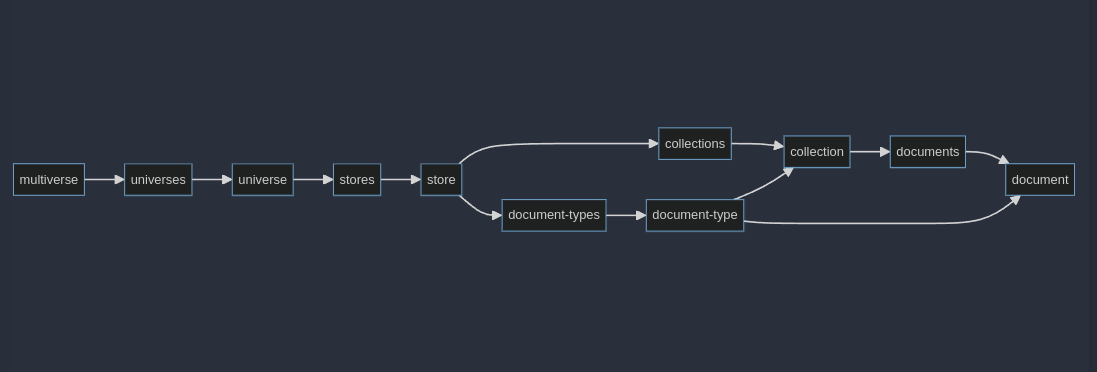
\includegraphics[width=.9\linewidth]{multiverse.png}
\end{center}

\subsubsection{Multiverse}
\label{sec:org00eb225}

A multiverse is the top structural container for data. A multiverse
contains one or more universes. A multiverse could be viewed as a
clustering of clusters of databases.

\subsubsection{Universe}
\label{sec:org1091a2f}

A universe contains one or more stores. A universe could be viewed as
a cluster of databases.

\subsubsection{Store}
\label{sec:org425c26f}

A store contains one or more collections. A store could be viewed as a database.

A store also contains one or more document-types.

\subsubsection{Document Type}
\label{sec:org264c208}

Document types are type schemas. A collection can be linked to a document-type. However
not all document-types have a direct link to a collection. Some
document types are indirectly linked because they are part of a
document with a hierarchical structure.

\subsubsection{Collection}
\label{sec:orgac5363c}

When data is persisted the file folders/directories mirror the
relationship above, which makes it possible to lazy load the data only
when needed from disk. Querying an unloaded collection will cause the
loading of a collection and in the case of naive-documents any
referenced collections as well.

\subsubsection{Documents}
\label{sec:orgb6b3b5e}

A document in \texttt{cl-naive-store} in simplest terms is a list of key
value pairs, in other words a property list. This is also how a
document is represented in the actual log files. Log files are read
using cl read-line.

\texttt{naive-indexed} adds the concept of a UUID (aka hash key).

\texttt{naive-documents} adds additional meta data like the multiverse,
universe, store, collection, changed data and old versions to the
document.

\subsection{In memory}
\label{sec:org32c8bcc}

Data is loaded into memory for querying and lookups, that makes them
fast.

You can load the whole multiverse, universe, a store, a collection or a shard at a
time.

\subsection{Lazy Loading}
\label{sec:orgb48b9a1}

You do not have to explicitly load data into memory upfront. You can
leave it up to the store to only load data when needed. It means that
you will only have the data that users requested up to that point in
memory. Data in memory can easily be garbage collected if not in use
any more. \texttt{cl-naive-store} does not do garbage collection for you that
is left to the user.

\subsection{Persistence}
\label{sec:orga90bc66}

\texttt{cl-naive-store} relies on the fact that objects are translatable to
key-value pairs and writes plists to a file per collection. Note of
caution here if you go and store unprintable values (ie not readable)
in the db you are going to be very disappointed when you try to load
the db again!

\subsection{Sharding}
\label{sec:org2f0fb64}

Sharding is the breaking down of files into smaller files, in the case
of naive-store that means that instead of one file per collection there
could be many.

Sharding is done based on the actual data in collections. The user
specifies which elements of a document it wants to use for sharding on
a collection. If none is specified no sharding is done.

You should not set up sharding to use data that can change for a
document, it will cause problems. For instance if you use company
name to affect sharding for data by company/client then you should not
be able to change the company name for the document. If you need to do
it on rare occasions then you should delete (and write out a new log
file with those documents stripped out) to keep your sanity.

\subsection{Document Types}
\label{sec:orgb508a12}

\texttt{cl-naive-store} is mostly/blissfully unaware of user defined document
types and value types. \texttt{document-types} adds document-type and element
classes, extending the store and collection classes to store document
types.

Document types are ignored when doing persistence, and loading from
disk, \texttt{document-types} just adds a place to store your document
types and retrieve them at run time. Document types can be what ever
you dream up!

If you want document type validation based on your document type
definitions you need to implement it yourself, overriding add-object
and persist-object should be enough.

\subsection{Definitions}
\label{sec:org4a214b3}

\texttt{cl-naive-store} stores definitions (plist trees) for multiverse,
universe, store, collection and document-types. These can be user to
load of a multiverse with minimal code instead of loading the store in
code steps.

You can use \texttt{definitions} to define the full multiverse schema.

\subsection{Naive Documents}
\label{sec:org4becc92}

Naive Documents uses \texttt{naive-core}, \texttt{naive-indexed}, \texttt{document-types}
and \texttt{definitions} to create a more complex/fleshed out data store
experience. Note that document types are still only used for their key
and index definitions and no data type specific validation is done
when loading or persisting data.

Other peculiarities of Naive Documents:

\begin{itemize}
\item Nothing stops you form adding "new" key values/types to your
document at any time, since they are not validated against a
document-type definition. A typical document database should be able
to store different document types or at least document-types with
varying data.
\item A document has key-values that are used to check for equality when
adding an object to a collection
\item A document keeps a set of old and new values while you are updating
values, this is cleared on persist.
\item A document is expected to be hierarchical in nature, i.e. a document
key-value pair can hold other documents (child documents). Child
documents come in two basic flavours, documents that have no
collection of their own (associated documents), and documents
referenced from other collections (reference documents). When a top
level document is persisted only "references" to the referenced
child document are persisted (The child document itself is not
updated!). Associated documents are persisted in full.
\end{itemize}

\subsection{BLOBS}
\label{sec:orgd76f9e9}

\texttt{cl-naive-store} knows how to deal with values that are blobs. Basically
blobs are written to their own files and if file type is relevant the
correct file type is used.

There are no tests for blobs yet so use at own risk!

\href{home.org}{Home} :noexport: \href{releases.org}{Previous} :noexport: \href{examples.org}{Next} :noexport:
\section{Definitions}
\label{sec:org86ff536}

Definitions should always be a valid plist if you want to use the
functions in naive-core to manipulate them.

This is the overview of what a full schema should look like.

\begin{verbatim}
(:multiverse
 [attributes]
 :universes ((:universe
              [attributes]
              :stores ((:store
                        [attributes]
                        :collections ((:collection
                                       ([attributes])))
                        :document-types ((:document-type
                                          [attributes]
                                          :elements ((:element ([attributes]))))))))))
\end{verbatim}

[attributes] roughly maps to slots from the related classes. Not all
slots are supported. Having a long hard look at the classes and the
examples will give you a good idea of which slots are supported. If
you are still not sure have a look at add-definition-element code for
each type of element.

You can add, remove and persist elements of definitions.

Have a look at the api documentation for:

\begin{itemize}
\item persist-definition

A definition is created from the data base object element passed and
stored with the data in the appropriate directory for its level.

\item add-definition-element
\item remove-definition-element
\end{itemize}

To load a store from a definition you can use load-from-definition.

Have a look at the \href{definitions-example.org}{example} and tests/test-definitions.lisp to learn
more about how to use definitions.

\section{Examples}
\label{sec:org42b61b0}

Examples below become more and more complex as you go down the list.

\subsection{Schema Definitions Example}
\label{sec:orgf69dc69}

Shows how to create a multiverse from a definition.

\begin{verbatim}
(ignore-errors (delete-package :naive-examples))

(require 'cl-naive-store.naive-documents)

(defpackage :naive-examples
  (:use :cl :cl-naive-store.naive-documents))

(in-package :naive-examples)

(defun example-location ()
  (cl-fad:merge-pathnames-as-directory
   (user-homedir-pathname)
   (make-pathname :directory (list :relative "multiverse"))))

;;Deleting existing example database
(cl-fad:delete-directory-and-files
 "~/multiverse/universe/simple-store"
 :if-does-not-exist :ignore)

(defvar *multiverse-definition*
  `(:multiverse
    (:name "multiverse"
     :universe-class cl-naive-store.naive-core:universe
     :location ,(example-location)
     :universes

     ((:universe
       (:name "universe"
        :location ,(cl-fad:merge-pathnames-as-directory
                    (example-location)
                    (make-pathname :directory (list :relative "universe")))
        ;;Universe classes can be specific to a universe.
        :universe-class cl-naive-store.naive-core:universe
        :store-class cl-naive-store.naive-documents:document-store
        :collection-class cl-naive-store.naive-documents:document-collection
        :document-type-class cl-naive-store.document-types:document-type
        :stores ((:store
                  (:name "human-resources"
                   :collections ((:collection
                                  (:name "laptops"
                                   :label "Laptops"
                                   :document-type "laptop"))
                                 (:collection
                                  (:name "employees"
                                   :label "Employees"
                                   :document-type "employee")))
                   :document-types
                         ((:document-type
                           (:name "laptop"
                            :label "Laptop"
                            :elements ((:element
                                        (:name :id
                                         :label "Serial No"
                                         :key-p t
                                         :concrete-type (:type :string)
                                         :attributes ((:attribute
                                                       (:name :display
                                                        :value t))
                                                      (:attribute
                                                       (:name :editable
                                                        :value t)))
                                         :documentation "Unique no that identifies the laptop."))
                                       (:element
                                        (:name :make
                                         :label "Manufaturer"
                                         :concrete-type (:type :string)
                                         :attributes ((:attribute
                                                       (:name :display
                                                        :value t))
                                                      (:attribute
                                                       (:name :editable
                                                        :value t)))
                                         :documentation "Then manufaturer of the laptop."))
                                       (:element (:name :model
                                                  :label "Model"
                                                  :concrete-type (:type :string)
                                                  :attributes ((:attribute
                                                                (:name :display
                                                                 :value t))
                                                               (:attribute
                                                                (:name :editable
                                                                 :value t)))
                                                  :documentation "Model of the laptop.")))
                            :attributes ()
                            :documentation "List of laptops the company owns."))

                          (:document-type
                           (:name "child"
                            :label "Child"
                            :elements ((:element
                                        (:name :name
                                         :label "Name"
                                         :key-p t
                                         :concrete-type (:type :string)
                                         :attributes ((:attribute
                                                       (:name :display
                                                        :value t))
                                                      (:attribute
                                                       (:name :editable
                                                        :value t)))
                                         :documentation "Name of child"))
                                       (:element
                                        (:name :sex
                                         :label "Gender"
                                         :concrete-type (:type :keyword)
                                         :attributes ((:attribute
                                                       (:name :display
                                                        :value t))
                                                      (:attribute
                                                       (:name :editable
                                                        :value t))
                                                      (:attribute
                                                       (:name :value-list
                                                        :value (:male :female))))
                                         :documentation "Gender of the child, can only be male or female."))
                                       (:element
                                        (:name :age
                                         :label "Age"
                                         :concrete-type (:type :number)
                                         :attributes
                                               ((:attribute
                                                 (:name :display
                                                  :value t))
                                                (:attribute
                                                 (:name :editable
                                                  :value t))
                                                (:attribute
                                                 (:name :setf-validate
                                                  :value
                                                        (lambda (age)
                                                          (if (<= age 21)
                                                              (values t nil)
                                                              (values nil "Child is to old"))))))
                                         :documentation "How old the child is")))
                            :attributes ()
                            :documentation "List of laptops the company owns."))

                          (:document-type
                           (:name "employee"
                            :label "Employee"
                            :elements ((:element
                                        (:name :emp-
                                         :label "Employee Number"
                                         :key-p t
                                         :concrete-type (:type :number)
                                         :attributes ((:attribute
                                                       (:name :display
                                                        :value t))
                                                      (:attribute
                                                       (:name :editable
                                                        :value t)))
                                         :documentation "Unique identifier of employee."))
                                       (:element (:name :name
                                                  :label "Name"
                                                  :concrete-type (:type :string)
                                                  :attributes ((:attribute
                                                                (:name :display
                                                                 :value t))
                                                               (:attribute
                                                                (:name :editable
                                                                 :value t)))
                                                  :documentation "Name of employee"))
                                       (:element
                                        (:name :sex
                                         :label "Gender"
                                         :concrete-type (:type :keyword)
                                         :attributes
                                               ((:attribute
                                                 (:name :display
                                                  :value t))
                                                (:attribute
                                                 (:name :editable
                                                  :value t))
                                                (:attribute
                                                 (:name :value-list
                                                  :value (:male :female))))

                                         :documentation "Gender of the child, can only be male or female."))
                                       (:element
                                        (:name :dependents
                                         :label "Children"
                                         :concrete-type (:type :list
                                                         :spec (:type :document
                                                                :spec (:type "child"
                                                                       :accessor (:name))))

                                         :attributes ((:attribute
                                                       (:name :display
                                                        :value t))
                                                      (:attribute
                                                       (:name :editable
                                                        :value t)))
                                         :documentation "List of the employees children"))
                                       (:element
                                        (:name :laptop
                                         :label "Laptop"
                                         :concrete-type (:type :document
                                                         :spec (:type "laptop"
                                                                :collection "laptop-collection"
                                                                :accessor (:id)))

                                         :attributes ((:attribute
                                                       (:name :display
                                                        :value t))
                                                      (:attribute
                                                       (:name :editable
                                                        :value t)))
                                         :documentation "Laptop allocated to employee"))
                                       (:element
                                        (:name :first-born
                                         :label "First Born Child"
                                         :concrete-type (:type :document
                                                         :spec (:type "child"
                                                                :collection "employees"
                                                                :accessor (:emp-no :dependents :name)))

                                         :attributes ((:attribute
                                                       (:name :display
                                                        :value t))
                                                      (:attribute
                                                       (:name :editable
                                                        :value t)))
                                         :documentation "List of the employees children")))
                            :attributes ()
                            :documentation "List of laptops the company owns."))))))))))))

(defparameter *multiverse* nil)

(setf *multiverse* (cl-naive-store.naive-core:load-from-definition
                    nil :multiverse *multiverse-definition* :with-children-p t))

;;Interogate multiverse
(break "~S" *multiverse*)

\end{verbatim}

\href{home.org}{Home} :noexport: \href{exmamples.org}{Previous} :noexport: \href{basic-example.org}{Next​} :noexport:
\subsection{Basic Example}
\label{sec:orgdbc5e3c}

In this example uses \texttt{naive-core} only, ie. the bare minimum
functionality. Documents \textbf{\textbf{are not persisted}} in this example. There are
use cases where the store can be used as kind of temporary database.

\begin{verbatim}
(ignore-errors (delete-package :naive-examples))

;;Load to use cl-naive-store
(require 'cl-naive-store)

(defpackage :naive-examples (:use :cl :cl-getx :cl-naive-store.naive-core))
(in-package :naive-examples)

;;Required to correctly initialize lparallel:*kernel*.
(initialize)


;;Deleting existing example database
(cl-fad:delete-directory-and-files
 "~/multiverse/universe/simple-store"
 :if-does-not-exist :ignore)

(let* (;;Create a multiverse.
       (multiverse (make-instance
                    'multiverse
                    :name "multiverse"
                    :location "~/multiverse/" ;Setting the location on disk.
                    :universe-class 'universe))
       ;;Create a universe and add it to the multiverse
       (universe (add-multiverse-element
                  multiverse
                  (make-instance
                   'universe
                   :name "universe"
                   :multiverse multiverse
                   :location "~/multiverse/universe/" ;Setting the location on disk.
                   :store-class 'store)))
       ;;Create a store and add it to the universe
       (store (add-multiverse-element
               universe
               (make-instance 'store
                              :name "simple-store"
                              :collection-class 'collection)))

       ;;Create a collection and add it to the store
       (collection (add-multiverse-element
                    store
                    (make-instance 'collection
                                   :name "simple-collection"
                                   ;;Specifying the key element, else its :key
                                   :keys '(:id)))))

  ;;Add some documents to the collection
  (add-document collection (list :name "Piet" :surname "Gieter" :id 123))
  (add-document collection (list :name "Sannie" :surname "Gieter" :id 321))
  (add-document collection (list :name "Koos" :surname "Van" :id 999))

  ;;Duplicates are handled by default, so this will not cause a duplicate document
  (add-document collection (list :name "Piet" :surname "Gieter" :id 123))

  ;;Query the collection
  (query-data collection :query (lambda (document)
                                  (<= (getx document :id) 900))))
\end{verbatim}

Output:

You can see that Piet Gieter appears only once, because duplicates are handled.

\begin{verbatim}
((:NAME "Piet" :SURNAME "Gieter" :ID 123)
 (:NAME "Sannie" :SURNAME "Gieter" :ID 321))
\end{verbatim}

To allow duplicates you need to set handle-duplicates-p to nil when
adding, persisting and loading the data.

\href{home.org}{Home} :noexport: \href{definitions-example.org}{Previous} :noexport: \href{basic-example-with-persistence.org}{Next} :noexport:
\subsection{Basic Example with Persistence}
\label{sec:org0009360}

In this example only the bare minimum is used and documents added are \textbf{\textbf{persisted}}.

\begin{verbatim}
(ignore-errors (delete-package :naive-examples))

;;Load to use cl-naive-store
(require 'cl-naive-store)
(defpackage :naive-examples (:use :cl :cl-getx :cl-naive-store.naive-core))
(in-package :naive-examples)

;;Required to correctly initialize lparallel:*kernel*.
(initialize)

;;Deleting existing example database
(cl-fad:delete-directory-and-files
 "~/multiverse/universe/simple-store"
 :if-does-not-exist :ignore)

(let* (;;Create a multiverse.
       (multiverse (make-instance
                    'multiverse
                    :name "multiverse"
                    :location "~/multiverse/" ;Setting the location on disk.
                    :universe-class 'universe))
       ;;Create a universe and add it to the multiverse
       (universe (add-multiverse-element
                  multiverse
                  (make-instance
                   'universe
                   :name "universe"
                   :multiverse multiverse
                   :location "~/multiverse/universe/" ;Setting the location on disk.
                   :store-class 'store)))
       ;;Create a store and add it to the universe
       (store (add-multiverse-element
               universe
               (make-instance 'store
                              :name "simple-store"
                              :collection-class 'collection)))

       ;;Create a collection and add it to the store
       (collection (add-multiverse-element
                    store
                    (make-instance 'collection
                                   :name "simple-collection"
                                   ;;Specifying the key element, else its :key
                                   :keys '(:id)))))

  ;;Add some documents to the collection
  (persist-document collection (list :name "Piet" :surname "Gieter" :id 123))
  (persist-document collection (list :name "Sannie" :surname "Gieter" :id 321))
  (persist-document collection (list :name "Koos" :surname "Van" :id 999))

  ;;Clear the collection, ie unload documents from memory so we can
  ;;show that it has been persisted.
  (clear-collection collection)

  ;;Query the collection, query-data will load the data from file if
  ;;the collection is empty
  (query-data collection :query (lambda (document)
                                  (<= (getx document :id) 900))))
\end{verbatim}

Output:

\begin{verbatim}
((:NAME "Piet" :SURNAME "Gieter" :ID 123)
 (:NAME "Sannie" :SURNAME "Gieter" :ID 321))
\end{verbatim}

To see the file created for the data go to
\textasciitilde{}/multiverse/universe/simple-store/simple-collection/ there you should
find a simple-collection.log file and you should see the following in
the file

\begin{verbatim}
(:NAME "Piet" :SURNAME "Gieter" :ID 123)
(:NAME "Sannie" :SURNAME "Gieter" :ID 321)
\end{verbatim}

\subsubsection{Lazy Loading}
\label{sec:orgbc8816b}

In this example \texttt{query-data} loaded and persisted (in one step) the
data into the collection. To show that the data was successfully
persisted and that query will lazy load the data when needed, the
collection is cleared and only then queried. 

You can explicitly load the collection yourself by using \texttt{(load-data collection)}.

\href{home.org}{Home} :noexport: \href{basic-example.org}{Previous} :noexport: \href{indexed-example.org}{Next} :noexport:
\subsection{Indexed Example}
\label{sec:org009f10a}

In this example we extend the basic functionality with indexing.

\begin{verbatim}
;;Load to use cl-naive-store
(require 'cl-naive-store)
(defpackage :naive-examples (:use :cl :cl-getx :cl-naive-store.naive-core
                             :cl-naive-store.naive-indexed))
(in-package :naive-examples)

;;Required to correctly initialize lparallel:*kernel*.
(initialize)

;;Deleting existing example database
(cl-fad:delete-directory-and-files
 "~/multiverse/universe/simple-store"
 :if-does-not-exist :ignore)

;;Create a class that inherits form indexed-collection-mixin and collection.
(defclass indexded-collection (indexed-collection-mixin collection)
  ())

(let* (;;Create a multiverse.
       (multiverse (make-instance
                    'multiverse
                    :name "multiverse"
                    :location "~/multiverse/" ;Setting the location on disk.
                    :universe-class 'universe))
       ;;Create a universe and add it to the multiverse
       (universe (add-multiverse-element
                  multiverse
                  (make-instance
                   'universe
                   :name "universe"
                   :multiverse multiverse
                   :location "~/multiverse/universe/" ;Setting the location on disk.
                   :store-class 'store)))
       ;;Create a store and add it to the universe
       (store (add-multiverse-element
               universe
               (make-instance 'store
                              :name "simple-store"
                              :collection-class 'indexed-collection)))

       ;;Create a collection and add it to the store
       (collection (add-multiverse-element
                    store
                    (make-instance 'indexed-collection
                                   :name "simple-collection"
                                   ;;Specifying the key element, else its :key
                                   :keys '(:id)
                                   ;; Specifying the elements to set up indexes for.
                                   :indexes '((:name :surname)))))
       (results))

  ;;Load Collection if it was created before.
  ;; (load-data collection)

  ;;Add some documents to the collection

  (persist-document collection (list :name "Piet" :surname "Gieter" :id 123))
  (persist-document collection (list :name "Sannie" :surname "Gieter" :id 321))
  (persist-document collection (list :name "Koos" :surname "Van" :id 999))
  (persist-document collection (list :name "Frikkie" :surname "Frikkedel" :id 1001))
  (persist-document collection (list :name "Tannie" :surname "Frikkedel" :id 1002))

  ;;Lookup koos using index values and add it to results
  (push
   (index-lookup-values collection (list (list :name "Koos")
                                         (list :surname "Van")))
   results)

  ;;Lookup Frikkedel using index values and add it to results
  (push
   (index-lookup-values collection (list :surname "Frikkedel"))
   results)

  ;;Query the collection, query-data will load the data from file if the collection is empty,
  ;;and add it to the results
  (push (query-data collection :query (lambda (document)
                                        (<= (getx document :id) 900)))
        results)

  (reverse results))

\end{verbatim}

Output:

;; Hashes will obviously be different for you.

\begin{verbatim}
((:DESC "Looked up Piet using index-lookup-hash." :VALUE
 (:NAME "Piet" :SURNAME "Gieter" :ID 123 :HASH
  "AB2CBF3C-41AE-4656-BE03-B360BCF6A707"))
(:DESC
 "Koos that we looked up using index-lookup-values and the index values of Koos and Van."
 :VALUE
 ((:NAME "Koos" :SURNAME "Van" :ID 999 :HASH
   "693A8B07-046E-4643-8FB2-926A965424BF")))
(:DESC
 "A list of both Frikie and Tannie that we looked up using index-lookup-values and the surname. This is called a partial index lookup. You can enable or disable partial indexes."
 :VALUE
 ((:NAME "Tannie" :SURNAME "Frikkedel" :ID 1002 :HASH
   "44A3BF6E-57C4-40BF-8692-54241564611D")
  (:NAME "Frikkie" :SURNAME "Frikkedel" :ID 1001 :HASH
   "5C7E02C7-3674-45FE-94A9-0B843478BA5E")))
(:DESC
 "Queried all id's <= 900 using query-data. The query will use indexes internally when possible."
 :VALUE
 ((:NAME "Sannie" :SURNAME "Gieter" :ID 321 :HASH
   "D0F597B2-12A2-4E05-971C-65B44F5CD4C4")
  (:NAME "Piet" :SURNAME "Gieter" :ID 123 :HASH
   "AB2CBF3C-41AE-4656-BE03-B360BCF6A707"))))
\end{verbatim}


\href{home.org}{Home} :noexport: \href{basic-example-with-persistence.org}{Previous} :noexport: \href{documents-example.org}{Next} :noexport:
\subsection{Naive Documents Example}
\label{sec:org069272d}

Using \texttt{cl-naive-store.naive-documents} gives you a lot of functionality out of the
box, but you need to do more work to set it up right.

\begin{verbatim}
(ignore-errors (delete-package :naive-examples))

;;Setup to use cl-naive-store
(require 'cl-naive-store)
(defpackage :naive-examples (:use
                             :cl
                             :cl-getx :cl-naive-store.naive-core
                             :cl-naive-store.naive-indexed
                             :cl-naive-store.document-types
                             :cl-naive-store.naive-documents))
(in-package :naive-examples)

;;Required to correctly initialize lparallel:*kernel*.
(initialize)

;;Deleting existing example database
(cl-fad:delete-directory-and-files
 "~/multiverse/universe/simple-store"
 :if-does-not-exist :ignore)

;;Create a data definition for an employee
;;It looks like a lot but dont panic its simple.
(defparameter *employee-document-type*
  '(:document-type (:name "employee"
                    :label "Employee"
                    :elements
                    ((:element
                      (:name :emp-no
                       :label "Employee No"
                       :key-p t
                       :concrete-type :string
                       :attributes ((:attribute
                                     (:name :display
                                      :value t))
                                    (:attribute
                                     (:name :editable
                                      :value t)))))
                     (:element
                      (:name :name
                       :label "Name"
                       :concrete-type :string
                       :attributes ((:attribute
                                     (:name :display
                                      :value t))
                                    (:attribute
                                     (:name :editable
                                      :value t)))))
                     (:element
                      (:name :surname
                       :label "Surname"
                       :concrete-type :string
                       :attributes ((:attribute
                                     (:name :display
                                      :value t))
                                    (:attribute
                                     (:name :editable
                                      :value t))))))
                    :documentation "This type represents a simple employee master.")))

(let* (;;Create Multiverse
       (multiverse
         (make-instance
          'multiverse
          :name "multiverse"
          :location "~/multiverse/" ;Setting the location on disk.
          :universe-class 'universe))
       ;;Add universe to multiverse
       (universe
         (add-multiverse-element
          multiverse
          (make-instance
           'universe
           :name "universe"
           :multiverse multiverse
           :location "~/multiverse/universe/" ;Setting the location on disk.
           :store-class 'document-store)))
       (store
         (add-multiverse-element
          universe
          (make-instance (store-class universe)
                         :name "simple-store"
                         :collection-class
                         'cl-naive-store.naive-documents:document-collection)))
       (document-type
         (load-from-definition
            store
            :document-type
            *employee-document-type*
            :with-children-p t))
       (collection (add-multiverse-element
                    store
                    (make-instance (collection-class store)
                                   :name "simple-collection"
                                   :document-type document-type
                                   ;; Not specifying the keys to show
                                   ;; that they are retrieved from the document-type
                                   ;; if if no key is set.
                                   ;; :keys ...
                                   ;; Specifying the elements to set up indexes for.
                                   :indexes '((:name :surname)))))
       ;;Add doc to collection
       (doc (persist-document collection
                              (make-document
                               :store (store collection)
                               :collection collection
                               :document-type "employee"
                               :elements (list :name "Piet" :surname "Gieter"
                                               :emp-no 123))))
       (results))

  ;;Persist store definition with its document type and collection.
  (persist multiverse :definitions-only-p t)

  ;;Add some documents to the collection

  (persist-document collection
                    (make-document
                     :store (store collection)
                     :collection collection
                     :document-type "employee"
                     :elements (list :name "Sannie" :surname "Gieter" :emp-no 321)))

  (persist-document collection
                    (make-document
                     :store (store collection)
                     :collection collection
                     :document-type "employee"
                     :elements (list :name "Koos" :surname "Van" :emp-no 999)))

  (persist-document collection
                    (make-document
                     :store (store collection)
                     :collection collection
                     :document-type "employee"
                     :elements (list :name "Frikkie" :surname "Frikkedel" :emp-no 1001)))

  (persist-document collection
                    (make-document
                     :store (store collection)
                     :collection collection
                     :document-type "employee"
                     :elements (list :name "Tannie" :surname "Frikkedel" :emp-no 1002)))

  ;;Look up piet by hash
  (push (list :desc "Looked up Piet using index-lookup-hash."
              :value (index-lookup-hash collection (getx doc :hash)))
        results)

  ;;Lookup koos using index values and add it to results
  (push
   (list :desc "Koos that we looked up using index-lookup-values and the index values of Koos and Van."
         :value
         (index-lookup-values collection (list (list :name "Koos")
                                               (list :surname "Van"))))
   results)

  ;;Lookup Frikkedel using index values and add it to results
  (push
   (list :desc "A list of both Frikie and Tannie that we looked up using index-lookup-values and the surname. This is called a partial index lookup. You can enable or disable partial indexes."
         :value
         (index-lookup-values collection (list :surname "Frikkedel")))
   results)

  ;;Query the collection, query-data will load the data from file if
  ;;the collection is empty, and add it to the results
  (push
   (list :desc "Queried all id's <= 900 using query-data. The query will use indexes internally when possible."
         :value
         (query-data collection :query (lambda (document)
                                         (<= (getx document :emp-no) 900))))
   results)

  (reverse results))
\end{verbatim}

Output:

\begin{verbatim}
((:DESC "Looked up Piet using index-lookup-hash." :VALUE
  #S(DOCUMENT
     :UNIVERSE #<UNIVERSE (:NAME "universe" :MULTIVERSE "multiverse" :LOCATION
                           "~/multiverse/universe/" :STORES
                           ("simple-store")) {104C234E83}>
     :STORE #<DOCUMENT-STORE (:NAME "simple-store" :UNIVERSE "universe"
                              :LOCATION #P"~/multiverse/universe/simple-store/"
                              :COLLECTIONS ("simple-collection")) {104C2B6C03}>
     :COLLECTION #<DOCUMENT-COLLECTION (:NAME "simple-collection" :STORE
                                        "simple-store" :LOCATION
                                        #P"~/multiverse/universe/simple-store/simple-collection/simple-collection.log"
                                        :DOCUMENT-TYPE "employee" :SHARDS
                                        ("simple-c")) {104C411AC3}>
     :DOCUMENT-TYPE "employee"
     :HASH "B58F9362-BDE0-465C-9013-04BF6541C8F7"
     :ELEMENTS (:NAME "Piet" :SURNAME "Gieter" :EMP-NO 123)
     :CHANGES NIL
     :VERSIONS NIL
     :DELETED-P NIL
     :PERSISTED-P T))
 (:DESC
  "Koos that we looked up using index-lookup-values and the index values of Koos and Van."
  :VALUE
  (#S(DOCUMENT
      :UNIVERSE #<UNIVERSE (:NAME "universe" :MULTIVERSE "multiverse" :LOCATION
                            "~/multiverse/universe/" :STORES
                            ("simple-store")) {104C234E83}>
      :STORE #<DOCUMENT-STORE (:NAME "simple-store" :UNIVERSE "universe"
                               :LOCATION
                               #P"~/multiverse/universe/simple-store/"
                               :COLLECTIONS
                               ("simple-collection")) {104C2B6C03}>
      :COLLECTION #<DOCUMENT-COLLECTION (:NAME "simple-collection" :STORE
                                         "simple-store" :LOCATION
                                         #P"~/multiverse/universe/simple-store/simple-collection/simple-collection.log"
                                         :DOCUMENT-TYPE "employee" :SHARDS
                                         ("simple-c")) {104C411AC3}>
      :DOCUMENT-TYPE #<DOCUMENT-TYPE (:NAME "employee" :STORE "simple-store"
                                      :ELEMENTS
                                      (:SURNAME :NAME :EMP-NO)) {104C2B6CA3}>
      :HASH "B0E59C8E-2241-490A-B904-1ABA62FD5C9B"
      :ELEMENTS (:NAME "Koos" :SURNAME "Van" :EMP-NO 999)
      :CHANGES NIL
      :VERSIONS NIL
      :DELETED-P NIL
      :PERSISTED-P T)))
 (:DESC
  "A list of both Frikie and Tannie that we looked up using index-lookup-values and the surname. This is called a partial index lookup. You can enable or disable partial indexes."
  :VALUE
  (#S(DOCUMENT
      :UNIVERSE #<UNIVERSE (:NAME "universe" :MULTIVERSE "multiverse" :LOCATION
                            "~/multiverse/universe/" :STORES
                            ("simple-store")) {104C234E83}>
      :STORE #<DOCUMENT-STORE (:NAME "simple-store" :UNIVERSE "universe"
                               :LOCATION
                               #P"~/multiverse/universe/simple-store/"
                               :COLLECTIONS
                               ("simple-collection")) {104C2B6C03}>
      :COLLECTION #<DOCUMENT-COLLECTION (:NAME "simple-collection" :STORE
                                         "simple-store" :LOCATION
                                         #P"~/multiverse/universe/simple-store/simple-collection/simple-collection.log"
                                         :DOCUMENT-TYPE "employee" :SHARDS
                                         ("simple-c")) {104C411AC3}>
      :DOCUMENT-TYPE #<DOCUMENT-TYPE (:NAME "employee" :STORE "simple-store"
                                      :ELEMENTS
                                      (:SURNAME :NAME :EMP-NO)) {104C2B6CA3}>
      :HASH "6BF9DC95-5158-4B60-A7E0-929BC2D7684F"
      :ELEMENTS (:NAME "Tannie" :SURNAME "Frikkedel" :EMP-NO 1002)
      :CHANGES NIL
      :VERSIONS NIL
      :DELETED-P NIL
      :PERSISTED-P T)
   #S(DOCUMENT
      :UNIVERSE #<UNIVERSE (:NAME "universe" :MULTIVERSE "multiverse" :LOCATION
                            "~/multiverse/universe/" :STORES
                            ("simple-store")) {104C234E83}>
      :STORE #<DOCUMENT-STORE (:NAME "simple-store" :UNIVERSE "universe"
                               :LOCATION
                               #P"~/multiverse/universe/simple-store/"
                               :COLLECTIONS
                               ("simple-collection")) {104C2B6C03}>
      :COLLECTION #<DOCUMENT-COLLECTION (:NAME "simple-collection" :STORE
                                         "simple-store" :LOCATION
                                         #P"~/multiverse/universe/simple-store/simple-collection/simple-collection.log"
                                         :DOCUMENT-TYPE "employee" :SHARDS
                                         ("simple-c")) {104C411AC3}>
      :DOCUMENT-TYPE #<DOCUMENT-TYPE (:NAME "employee" :STORE "simple-store"
                                      :ELEMENTS
                                      (:SURNAME :NAME :EMP-NO)) {104C2B6CA3}>
      :HASH "97DC3D26-97A9-4B75-A8A3-36B849CAE347"
      :ELEMENTS (:NAME "Frikkie" :SURNAME "Frikkedel" :EMP-NO 1001)
      :CHANGES NIL
      :VERSIONS NIL
      :DELETED-P NIL
      :PERSISTED-P T)))
 (:DESC
  "Queried all id's <= 900 using query-data. The query will use indexes internally when possible."
  :VALUE
  (#S(DOCUMENT
      :UNIVERSE #<UNIVERSE (:NAME "universe" :MULTIVERSE "multiverse" :LOCATION
                            "~/multiverse/universe/" :STORES
                            ("simple-store")) {104C234E83}>
      :STORE #<DOCUMENT-STORE (:NAME "simple-store" :UNIVERSE "universe"
                               :LOCATION
                               #P"~/multiverse/universe/simple-store/"
                               :COLLECTIONS
                               ("simple-collection")) {104C2B6C03}>
      :COLLECTION #<DOCUMENT-COLLECTION (:NAME "simple-collection" :STORE
                                         "simple-store" :LOCATION
                                         #P"~/multiverse/universe/simple-store/simple-collection/simple-collection.log"
                                         :DOCUMENT-TYPE "employee" :SHARDS
                                         ("simple-c")) {104C411AC3}>
      :DOCUMENT-TYPE "employee"
      :HASH "B94547F2-DEE5-4408-A6DB-459E193E0B22"
      :ELEMENTS (:NAME "Sannie" :SURNAME "Gieter" :EMP-NO 321)
      :CHANGES NIL
      :VERSIONS NIL
      :DELETED-P NIL
      :PERSISTED-P T)
   #S(DOCUMENT
      :UNIVERSE #<UNIVERSE (:NAME "universe" :MULTIVERSE "multiverse" :LOCATION
                            "~/multiverse/universe/" :STORES
                            ("simple-store")) {104C234E83}>
      :STORE #<DOCUMENT-STORE (:NAME "simple-store" :UNIVERSE "universe"
                               :LOCATION
                               #P"~/multiverse/universe/simple-store/"
                               :COLLECTIONS
                               ("simple-collection")) {104C2B6C03}>
      :COLLECTION #<DOCUMENT-COLLECTION (:NAME "simple-collection" :STORE
                                         "simple-store" :LOCATION
                                         #P"~/multiverse/universe/simple-store/simple-collection/simple-collection.log"
                                         :DOCUMENT-TYPE "employee" :SHARDS
                                         ("simple-c")) {104C411AC3}>
      :DOCUMENT-TYPE "employee"
      :HASH "B58F9362-BDE0-465C-9013-04BF6541C8F7"
      :ELEMENTS (:NAME "Piet" :SURNAME "Gieter" :EMP-NO 123)
      :CHANGES NIL
      :VERSIONS NIL
      :DELETED-P NIL
      :PERSISTED-P T))))
\end{verbatim}

To change a value for an employee you just set the value using
getx. For example lets change Sannie's surname.

\begin{verbatim}
(let ((sannie (first (index-lookup-values
                      (get-multiverse-element
                       :collection
                       (get-multiverse-element
                        :store
                        *universe* "simple-store")
                       "simple-collection")
                      (list (list :name "Sannie")
                            (list :surname "Gieter"))))))

  (setf (getx sannie :surname) "Potgieter"))
\end{verbatim}

Which will give you

\begin{verbatim}
#S(document
   :STORE #<document-STORE {10172A8A73}>
   :COLLECTION #<document-COLLECTION {1017369EA3}>
   :DATA-TYPE "employee"
   :HASH "68434DF1-A04D-4D33-96F1-89D217A193FD"
   :VALUES (:NAME "Sannie" :SURNAME "Gieter" :EMP-NO 321)
   :CHANGES (:NAME "Sannie" :SURNAME "Potgieter" :EMP-NO 321)
   :VERSIONS NIL
   :DELETED-P NIL
   :PERSISTED-P T)
\end{verbatim}

The update values can be found in :changes, and will stay there until
the document is persisted or abandoned.

Take note that \textbf{\textbf{getx}} will return "Potgieter" now even if the
document has not been persisted yet.

\href{home.org}{Home} :noexport: \href{indexed-example.org}{Previous} :noexport: \href{sharding-example.org}{Next} :noexport:
\subsection{Sharding Example}
\label{sec:org6790baf}

In this example we will use sharding with document types.

\begin{verbatim}
(ignore-errors (delete-package :naive-examples))

;;Setup to use cl-naive-store
(require 'cl-naive-store)
(defpackage :naive-examples (:use
                             :cl
                             :cl-getx :cl-naive-store.naive-core
                             :cl-naive-store.naive-indexed
                             :cl-naive-store.document-types
                             :cl-naive-store.naive-documents))
(in-package :naive-examples)

;;Required to correctly initialize lparallel:*kerel*.
(initialize)

(defparameter *surnames*
  #("Smith" "Johnson" "Williams" "Jones" "Brown" "Davis" "Miller")
  "A vector of surnames.")

(defparameter *countries*
  #("Afghanistan" "Albania" "Algeria" "Andorra" "Angola"
    "Antigua and Barbuda" "Argentina" "Armenia" "Australia" "Austria"
    "Azerbaijan" "Bahamas" "Bahrain" "Bangladesh" "Barbados" "Belarus"
    "Belgium" "Belize" "Benin" "Bhutan" "Bolivia" "Bosnia and Herzegovina"
    "Botswana" "Brazil" "Brunei" "Bulgaria" "Burkina Faso" "Burundi"
    "Côte d'Ivoire" "Cabo Verde" "Cambodia" "Cameroon" "Canada"
    "Central African Republic" "Chad" "Chile" "China" "Colombia" "Comoros"
    "Congo" "Costa Rica" "Croatia" "Cuba" "Cyprus"
    "Czechia" "Democratic Republic of the Congo"
    "Denmark" "Djibouti" "Dominica" "Dominican Republic" "Ecuador" "Egypt"
    "El Salvador" "Equatorial Guinea" "Eritrea" "Estonia"
    "Eswatini" "Ethiopia" "Fiji" "Finland" "France"
    "Gabon" "Gambia" "Georgia" "Germany" "Ghana" "Greece" "Grenada"
    "Guatemala" "Guinea" "Guinea-Bissau" "Guyana" "Haiti" "Holy See"
    "Honduras" "Hungary" "Iceland" "India" "Indonesia" "Iran" "Iraq"
    "Ireland" "Israel" "Italy" "Jamaica" "Japan" "Jordan" "Kazakhstan"
    "Kenya" "Kiribati" "Kuwait" "Kyrgyzstan" "Laos" "Latvia" "Lebanon"
    "Lesotho" "Liberia" "Libya" "Liechtenstein" "Lithuania" "Luxembourg"
    "Madagascar" "Malawi" "Malaysia" "Maldives" "Mali" "Malta"
    "Marshall Islands" "Mauritania" "Mauritius" "Mexico" "Micronesia"
    "Moldova" "Monaco" "Mongolia" "Montenegro" "Morocco" "Mozambique"
    "Myanmar" "Namibia" "Nauru" "Nepal" "Netherlands"
    "New Zealand" "Nicaragua" "Niger" "Nigeria" "North Korea"
    "North Macedonia" "Norway" "Oman" "Pakistan" "Palau" "Palestine State"
    "Panama" "Papua New Guinea" "Paraguay" "Peru" "Philippines" "Poland"
    "Portugal" "Qatar" "Romania" "Russia" "Rwanda" "Saint Kitts and Nevis"
    "Saint Lucia" "Saint Vincent and the Grenadines" "Samoa" "San Marino"
    "Sao Tome and Principe" "Saudi Arabia" "Senegal" "Serbia" "Seychelles"
    "Sierra Leone" "Singapore" "Slovakia" "Slovenia" "Solomon Islands"
    "Somalia" "South Africa" "South Korea" "South Sudan" "Spain"
    "Sri Lanka" "Sudan" "Suriname" "Sweden" "Switzerland" "Syria"
    "Tajikistan" "Tanzania" "Thailand" "Timor-Leste" "Togo" "Tonga"
    "Trinidad and Tobago" "Tunisia" "Turkey" "Turkmenistan" "Tuvalu"
    "Uganda" "Ukraine" "United Arab Emirates" "United Kingdom"
    "United States of America" "Uruguay" "Uzbekistan" "Vanuatu"
    "Venezuela" "Vietnam" "Yemen" "Zambia" "Zimbabwe")
  "A vector of country names.")

(defparameter *employee-document-type*
  '(:document-type (:name "employee"
                    :label "Employee"
                    :elements
                    ((:element
                      (:name :emp-no
                       :label "Employee No"
                       :key-p t
                       :concrete-type :string
                       :attributes ((:attribute
                                     (:name :display
                                      :value t))
                                    (:attribute
                                     (:name :editable
                                      :value t)))))
                     (:element
                      (:name :name
                       :label "Name"
                       :concrete-type :string
                       :attributes ((:attribute
                                     (:name :display
                                      :value t))
                                    (:attribute
                                     (:name :editable
                                      :value t)))))
                     (:element
                      (:name :surname
                       :label "Surname"
                       :concrete-type :string
                       :attributes ((:attribute
                                     (:name :display
                                      :value t))
                                    (:attribute
                                     (:name :editable
                                      :value t))))))
                    :documentation "This type represents a simple employee master.")))

;;Cannot go below 202! The tests will fail.
(defparameter *size* 10000)

(defparameter *expected-shard-count* 0)

;;Doing this so you can rerun the code from here onwards.
(progn
  ;;Deleting existing example database
  (cl-fad:delete-directory-and-files
   "~/multiverse/universe/simple-store"
   :if-does-not-exist :ignore)

  (let* ((multiverse
           (make-instance
            'multiverse
            :name "multiverse"
            :location "~/multiverse/" ;Setting the location on disk.
            :universe-class 'universe))
         ;;Add universe to multiverse
         (universe
           (add-multiverse-element
            multiverse
            (make-instance
             'universe
             :name "universe"
             :multiverse multiverse
             :location "~/multiverse/universe/" ;Setting the location on disk.
             :store-class 'document-store)))
         (store
           (add-multiverse-element
            universe
            (make-instance (store-class universe)
                           :name "simple-store"
                           :collection-class
                           'cl-naive-store.naive-documents:document-collection)))
         (document-type
           (make-instance
            'document-type
            :name (getf
                   (getf *employee-document-type* :document-type)
                   :name)
            :label (getf
                    (getf *employee-document-type* :document-type)
                    :label)
            :elements (mapcar
                       (lambda (element)
                         (make-instance
                          'element
                          :name(getf (getf element :element) :name)
                          :key-p (getf (getf element :element) :key-p)
                          :concrete-type (getf (getf element :element) :concrete-type)
                          :attributes (getf (getf element :element) :attributes)))
                       (getf
                        (getf *employee-document-type* :document-type)
                        :elements))))
         (collection
           (add-multiverse-element
            store
            (make-instance (collection-class store)
                           :name "simple-collection"
                           :keys '(:emp-no)
                           :document-type document-type
                           ;; Creating shards based on the country that the employee
                           ;; belongs to.  It is a bad example you should not shard on
                           ;; any value that could change in the future!
                           :shard-elements '(:country))))
         (emp-country  0)
         (emp-surname  0)
         (unique-countries (make-hash-table :test 'equalp)))

    (setf *expected-shard-count* 0)

    (cl-naive-store.naive-core:add-multiverse-element store document-type)

    (persist multiverse :definitions-only-p t)

    (unless (data-loaded-p collection)
      ;;Populate the collection.
      (dotimes (emp-no *size*)
        ;; We create employees country per country and loop again if we need more:
        (let ((country  (aref *countries* emp-country))
              (surname  (aref *surnames* emp-surname)))

          (unless (gethash country unique-countries)
            (incf *expected-shard-count*)
            (setf (gethash country unique-countries) country))

          (incf emp-surname)

          ;;We only have only 7 surnames start again on surnames
          (when (<= (length *surnames*) emp-surname)
            (setf emp-surname 0)
            ;;move on to next country
            ;;(setf emp-country (mod (1+ emp-country) (length *countries*)))
            (if (< emp-country (- (length *countries*) 1))
                (incf emp-country)
                (setf emp-country 0)))

          (add-document collection
                        (list
                         :country country
                         :surname surname
                         :name (format nil "Slave No ~A" emp-no)
                         :emp-no emp-no)
                        :handle-duplicates-p nil)))

      ;; Bulk perist documents
      (persist-collection collection))

    ;;We are just going to investigate the shards and not do a lot data
    ;;lookups like in other examples.
    (list (list :desc "Count of shards in collection."
                :value (length (shards collection)))
          (list :desc "The count of physical shard files for the collection."
                :value (length (uiop:directory-files
                                (cl-fad:merge-pathnames-as-directory
                                 (location store)
                                 (make-pathname :directory
                                                (list :relative
                                                      (name collection))))))))))

\end{verbatim}

Output:

\begin{verbatim}
((:DESC "Count of shards in collection." :VALUE 195)
 (:DESC "The count of physical shard files for the collection." :VALUE 195))
\end{verbatim}

\href{home.org}{Home} :noexport: \href{documents-example.org}{Previous} :noexport:

\section{User API}
\label{sec:org743234b}

The classes, accessors and generic functions used by the typical user
of cl-naive-store. Please have a look at the documentation and
examples for help on how to use cl-naive-store. The api documentation
only deals with the specifics of individual api functions. If you want
to cutsomize cl-naive-store then you need to use the functionality
described here in condjuction with the Implementor's Api.

\subsection{Naive Core}
\label{sec:orgd78be29}

\subsubsection{[generic function] query-definitions (definition \&key fn element)}
\label{sec:orga6810f8}

Queries the definition passed for an element or elements.

If an element is supplied limits calling the function to those elements or if no function is supplied just fetches elements of keyword element.

If you need more control use cl-naive-ptrees directly.

\subsubsection{[generic function] get-definition-element (element-type parent name)}
\label{sec:orgd05ff2e}

Fetches a definition of the type element-type by name from the parent definition.

\subsubsection{[generic function] add-definition-element (element-type definition element \&key name-path)}
\label{sec:org1995cdd}

Adds a definition element to the parent definition.

\begin{enumerate}
\item add-definition-element ((element-type (eql :collection)) definition collection \&key name-path replace-p)
\label{sec:org755324c}
\item add-definition-element ((element-type (eql :document-type)) definition collection \&key name-path replace-p)
\label{sec:orgafa1d28}
\item add-definition-element ((element-type (eql :store)) definition collection \&key name-path replace-p)
\label{sec:org5bd340d}
\item add-definition-element ((element-type (eql :universe)) definition collection \&key name-path replace-p)
\label{sec:org4612057}
\end{enumerate}

\subsubsection{[generic function] remove-definition-element (element-type definition element-name \&key name-path)}
\label{sec:org475b7a2}

Removes a definition element from the definition.

\begin{enumerate}
\item remove-definition-element ((element-type (eql :universe)) definition element-name \&key name-path)
\label{sec:org46a1541}
\item remove-definition-element ((element-type (eql :store)) definition element-name \&key name-path)
\label{sec:org84f847b}
\item remove-definition-element ((element-type (eql :collection)) definition element-name \&key name-path)
\label{sec:org52f1e0b}
\item remove-definition-element ((element-type (eql :document-type)) definition element-name \&key name-path)
\label{sec:orge4d6d32}
\end{enumerate}

\subsubsection{[function] get-definitions (location definition-type)}
\label{sec:org2db8141}

Returns persisted definitions for the type (multiverse, universe,
store, collection) using the passed object that can be a multiverse,
universe, store, collection.  If no definition-type is not supplied
the definition of the object is returned.

\subsubsection{[function] get-definition (location definition-type name \&key (error-p t))}
\label{sec:orgb599887}

Returns a persisted definition for the type (multiverse, universe,
store, collection) using the passed object that can be a multiverse,
universe, store, collection.

\subsubsection{[generic function] instance-from-definition (definition-type definition)}
\label{sec:org80dbd5d}

Instanciates an element from the definition for the likes of
multiverse, universe, store, collection or document-type.

This method has no knowledge of or ignores the existance of parents
and children elements.

\begin{enumerate}
\item instance-from-definition ((class (eql 'multiverse)) definition)
\label{sec:orgdcf4636}
\item instance-from-definition ((class (eql 'universe)) definition)
\label{sec:org43b53e0}
\item instance-from-definition ((class (eql 'store)) definition)
\label{sec:org725e542}
\item instance-from-definition ((class (eql 'collection)) definition)
\label{sec:orgc4f2096}
\item instance-from-definition ((class (eql 'document-type)) definition)
\label{sec:org6703cd7}
\end{enumerate}

\subsubsection{[generic function] load-from-definition (parent definition-type definition \&key class with-children-p with-data-p)}
\label{sec:orge56fb41}

Instanciates an element from the definition for the likes of
multiverse, universe, store, collection or document-type and loads it
into the multiverse using the parent.

Multiverse elements usually have a reference to the parent that needs
to be set. For instance a collection will have a reference to its
store.

Multiverse elements usually also have child elements that could be
instanciated for the relevent element. The choice is left up to the
user. If the user does want children to also be instanciated they can
supply a complete definition or rely on naive-store persisted
definition files to be found and used. Set with-children-p for the
required behaviour.

Whether documents (the actual data) is loaded after instanciation is a
choice of the user. Use with-data-p to affect the behaviour. Just note
that if you load data this way you are forgoing lazy loading.

\begin{enumerate}
\item load-from-definition ((multiverse multiverse) (definition-type (eql :universe)) definition \&key class with-children-p with-data-p)
\label{sec:orgfefa082}
\item load-from-definition ((universe universe) (definition-type (eql :store)) definition \&key class with-children-p with-data-p)
\label{sec:orge13cfff}
\item load-from-definition ((store store) (definition-type (eql :collection)) definition \&key class with-children-p with-data-p)
\label{sec:org820a297}
\item load-from-definition ((store store) (definition-type (eql :document-type)) definition \&key class with-children-p with-data-p)
\label{sec:org2c2bd81}
\end{enumerate}

\subsubsection{[generic function] load-from-definition-file (parent definition-type name \&key class with-children-p with-data-p)}
\label{sec:org3773e82}

Loads a definition from a file.

\subsubsection{[class] shard}
\label{sec:orge6e2c7e}

Sharding is when you break the physical file that backs the collection
into smaller files based on data elements of a document. An instance
of a shard class is used to load the documents belonging to the shard
into memory.

\begin{enumerate}
\item\relax [accessor] mac
\label{sec:orgd18eb7b}

Mac to identify shard.

\item\relax [accessor] location
\label{sec:orgef58fa1}

The file path to this shard is stored.

\item\relax [accessor] documents
\label{sec:orgef098ea}

Documents belonging to shard stored in an adjustable array.

\item\relax [accessor] status
\label{sec:org062f54e}

Used internally during the loading of the documents in a shard to help with locking.

\item\relax [accessor] lock
\label{sec:org9211506}

Used internally to do shard specific locking.
\end{enumerate}

\subsubsection{[class] multiverse}
\label{sec:orge51a8ab}

A multiverse is the top structural container for data. A multiverse
contains one or more universes. A multiverse could be viewed as a clustering of clusters of
databases.

\begin{enumerate}
\item\relax [accessor] name
\label{sec:org5dd19f3}

Mulitiverse name.

\item\relax [accessor] universes
\label{sec:org2bfe640}

List of universes contained by this multiverse.

\item\relax [accessor] universe-class
\label{sec:org432e866}

The class that should be used to make universes.

NOTES:

universe-class is delcaritively specied here because stores are
dynamicly created when definition files are loaded. (see store notes
for more about this.)

\item\relax [accessor] Location
\label{sec:org6ead46c}

The directory path to universes for this multiverse.
\end{enumerate}

\subsubsection{[class] universe}
\label{sec:org4c0d04e}

A universe contains one or more stores. A universe could be viewed as
a cluster of databases.

\begin{enumerate}
\item\relax [accessor] multiverse
\label{sec:org50ab24a}

The multiverse the universe belongs to.

\item\relax [accessor] name
\label{sec:orgea73418}

Universe name.

\item\relax [accessor] stores
\label{sec:org6566afd}

List of stores contained by this universe.

\item\relax [accessor] store-class
\label{sec:orge6015fa}

The class that should be used to make stores.

NOTES:

store-class is delcaritively specied here because stores are dynamicly
created when definition files are loaded. (see store notes for more
about this.)

\item\relax [accessor] location
\label{sec:orgd065645}

Directory path to stores of this universe.
\end{enumerate}

\subsubsection{[class] store}
\label{sec:orgbe5530f}

Document types and their associated collections are organized into
groups called stores.

NOTES:

collection-class and document-type-class is delcaritively specied here
because they are dynamicly created when definition files are
loaded. The alternative would be defmethod hell where the customizer
of naive-store would have to implement a whole lot of methods that do
exactly what the provided methods do just to be able to be type
specific in other methods where it is actually needed. Alternatively
meta classes could be used for element-class but that opens another
can of worms.

\begin{enumerate}
\item\relax [accessor] universe
\label{sec:org639c03d}

The universe the store belongs to.

\item\relax [accessor] name
\label{sec:org0ee63b8}

Store name.

\item\relax [accessor] collection-class
\label{sec:orgea4d968}

The class that should be used to make collections.

\item\relax [accessor] collections
\label{sec:orgf3f7c50}

List of collections represented by this store.

\item\relax [accessor] Location
\label{sec:org08be04e}

The directory path to the document-type files and collection files for
this store.
\end{enumerate}

\subsubsection{[class] collection}
\label{sec:org7884372}

A collection of documents of a specific document-type.

\begin{enumerate}
\item\relax [accessor] store
\label{sec:orgc7ff0a3}

The store that this collection belongs to.

\item\relax [accessor] name
\label{sec:orgc56328b}

The collection name.

\item\relax [accessor] location
\label{sec:orga7be04e}

The directory path to where files for this collection are stored.

\item\relax [accessor] shards
\label{sec:org4bdd781}

A vector of shards.

NOTES:

Originally naive-store used lists but with the re-introduction of
sharding, we chose to also introduce the use of lparrallel to speed
up many functions and lparrallel has a preference for arrays.

\item\relax [accessor] keys
\label{sec:org0890e31}

Keys need to be set to handle duplicates, the default is :key if :key
is not found in the document then duplicates will occur.

NOTES:

For collections that use cl-naive-document-type there is a fallback
the document-type is checked for keys as well and the collection's
keys will be set to the keys set in the document-type elements.

\item\relax [accessor] shard-elements
\label{sec:org5226156}

shard-elements is a list of document element keywords to use for sharding.
\end{enumerate}

\subsubsection{[method] documents ((collection collection))}
\label{sec:org9f53a2e}

It is a convenience function to retrieve all documents without having
to deal with shards.

Loops over all the shards for a collection to gather all the
documents.

\subsubsection{[method] getx and (setf getx)}
\label{sec:org57e35d9}

Implements getx for multiverse, universe, store and collection.

This means instead of ([accessor] object) you can use (getx object :[accessor]).

\subsubsection{[generic function] status (shard) and (setf status)}
\label{sec:org29caaf8}

Used to monitor shards during loading.

\begin{enumerate}
\item (setf status) (new-status (shard shard))
\label{sec:orgd78a32c}

\item status ((shard shard))
\label{sec:org84d153d}
\end{enumerate}

\subsubsection{[generic function] short-mac (shard)}
\label{sec:org92cfec0}

Return a short string containing a prefix of the MAC.

\begin{enumerate}
\item short-mac ((shard shard))
\label{sec:org5321723}
\end{enumerate}

\subsubsection{[function] match-shard (filename shards)}
\label{sec:org5bd3a3b}

Check filename against a list of shards to find the matching shard.

\subsubsection{[generic function] get-shard (collection shard-mac \&key \&allow-other-keys)}
\label{sec:orgb961e66}

Get the shard object by its mac. Shard lookups are done so much that
there is no choice but to cache them in a hashtable, but that
hashtable needs to be thread safe so using safe functions to get and
set.

\subsubsection{[generic function] make-shard (collection shard-mac))}
\label{sec:org8602c2d}
make-shard ((collection indexed-collection-mixin) shard-mac)

Creates an instance of a shard using the supplied mac.

\subsubsection{[function] document-shard-mac (collection document)}
\label{sec:org9d7c2bd}

Calculating a mac is expensive so caching shard value macs in a
hashtable but that hashtable needs to be thread safe so using safe
functions to get and set.

\subsubsection{[generic function] query-multiverse (element fn)}
\label{sec:orgfd9168a}

Queries the multiverse element passed for an element or elements.

\begin{enumerate}
\item query-multiverse ((collection collection) fn)
\label{sec:orgb1f19d5}

\item query-multiverse ((store store) fn)
\label{sec:org9b7bf39}

\item query-multiverse ((universe universe) fn)
\label{sec:org0f370ef}

\item query-multiverse ((multiverse multiverse) fn)
\label{sec:org0cb654b}
\end{enumerate}

\subsubsection{[generic function] get-multiverse-element (element-type parent name)}
\label{sec:org8fde332}

Fetches an element of the type with matching name.

\begin{enumerate}
\item get-multiverse-element ((element-type (eql :universe)) (multiverse multiverse) name)
\label{sec:org6c34042}

\item get-multiverse-element ((element-type (eql :store)) (universe universe) name)
\label{sec:org5a7e8c1}

\item get-multiverse-element ((element-type (eql :collection)) (store store) name)
\label{sec:org95db810}
\end{enumerate}

\subsubsection{[generic function] persist (object \&key \&allow-other-keys)}
\label{sec:orge1cdda0}

\begin{enumerate}
\item persist ((multiverse multiverse) \&key \&allow-other-keys)
\label{sec:org6b0ec84}

Persists a multiverse definition and not what it contains! Path to
file is of this general format /multiverse/multiverse-name.universe.

\item persist ((universe universe) \&key \&allow-other-keys)
\label{sec:org75d68d2}

Persists a universe definition and not what it contains! Path to file
is of this general format
/multiverse/universe-name/universe-name.universe.

\item persist ((store store) \&key \&allow-other-keys)
\label{sec:org2e9e535}

Persists a store definition and not what it contains! Path to file is
of this general format /universe/store-name/store-name.store.

\item persist ((collection collection) \&key \&allow-other-keys)
\label{sec:orge5a5119}

Persists a collection definition and the documents in a
collection. Path to file for data is this general format
/universe/store-name/collection-name/collection-name.log
\end{enumerate}

\subsubsection{[function] persist-collection (collection)}
\label{sec:org71f7a26}

Persists the documents in a collection in the order that they where
added.

\subsubsection{[generic function] add-multiverse-element (parent element \&key persist-p)}
\label{sec:org2792aba}

Adds an instance of a multiverse element to the parent instance.

\begin{enumerate}
\item add-multiverse-element ((multiverse multiverse) (universe universe))
\label{sec:org4938991}
\item add-multiverse-element ((universe universe) (store store))
\label{sec:org7109b4e}
\item add-multiverse-element ((store store) (collection collection))
\label{sec:orgea844d2}
\end{enumerate}

\subsubsection{[generic function] clear-collection (collection)}
\label{sec:orga3e9999}

Clears documents indexes etc from collection.

\subsubsection{[generic function] remove-multiverse-element (parent element)}
\label{sec:orgd59719c}

Removes an instance of a multiverse element from the parent instance.

\begin{enumerate}
\item remove-multiverse-element ((store store) (collection collection) \&key remove-data-from-disk-p)
\label{sec:org6a17525}
\item remove-multiverse-element ((multiverse multiverse) (universe universe) \&key)
\label{sec:org1bd6203}
\item remove-multiverse-element ((universe universe) (store store) \&key)
\label{sec:org9908900}
\end{enumerate}


\subsubsection{[generic function] load-data (collection \&key force-reload-p \&allow-other-keys)}
\label{sec:org7a43de9}

Loads the data documents of a collection from file or files if
sharding is used. If the data is already loaded it wont reload it.

shard-macs is a list of shard macs to indicate which shards should be
used. If no shards are specified all shards will be loaded.

\subsubsection{[generic function] ensure-location (object)}
\label{sec:org0e888d0}

Tries to find or build path to cl-naive-store files.

\begin{enumerate}
\item ensure-location ((object multiverse))
\label{sec:orgc194c02}
\item ensure-location ((object universe))
\label{sec:org35405bc}
\item ensure-location ((object store))
\label{sec:org0a68c63}
\item ensure-location ((object collection))
\label{sec:org25c9c4d}
\end{enumerate}

\subsubsection{[generic function] data-loaded-p (container \&key *allow-other-keys)}
\label{sec:org0683ada}

Checks if the data is loaded for the container, be it universe , store or collection.

NOTES:

This physically checks each collection's underlying concrete data structure for data. This is done because a collection can be empty and still loaded, thus setting a status when loaded became confusing and could be missed by an over loading method.

If you change the underlying container for (shards collection) or the
container for (docutments shard) you have to implement
data-loaded-p. Your implementation is expected to physically check for
document count > 0 and not some status set. Be smart about it you are
not expected to return a count so dont waist time counting just check
if there is at least one document in the container.


\begin{enumerate}
\item data-loaded-p ((collection collection) \&key \&allow-other-keys)
\label{sec:org64a7f69}

\item data-loaded-p ((store store) \&key \&allow-other-keys)
\label{sec:org5f20865}

\item data-loaded-p ((universe universe) \&key \&allow-other-keys)
\label{sec:org2f81ea9}
\end{enumerate}


\subsubsection{[generic function] document-values (document)}
\label{sec:orgad4aff9}

Returns a plist of document values.

NOTES:

Exists to ease the compatibility of various implementation
functions. Basically it blurs the line between plists and more complex
documents like cl-naive-store.naive-documents document struct.

This helps keep the amount of specializations needed down
considerably.

\begin{enumerate}
\item document-values (document)
\label{sec:org9a31d8a}

\item document-values ((document document))
\label{sec:org5d33297}
\end{enumerate}

\subsubsection{[generic function] key-values (collection values \&key \&allow-other-keys)}
\label{sec:orgbc22bef}

key-values ((collection collection) values \&key \&allow-other-keys)

Returns a set of key values from the values of a data document. Checks
the collection keys or uses hash.

\begin{enumerate}
\item key-values ((collection collection) values \&key \&allow-other-keys)
\label{sec:org9801a02}
\end{enumerate}

\subsubsection{[generic function] existing-document (collection document \&key shard \&allow-other-keys)}
\label{sec:org10fd1cb}

Finds any documents with the same key values. This could return the
exact same document or a similar document.

If a shard is passed in then the search is limited to that shard.

IMPL NOTES:

This is an essential part of loading and persisting documents, take
care when implementing.

\subsubsection{[generic function] deleted-p (document)}
\label{sec:org3e648b3}

(setf deleted-p) (value document \&key \&allow-other-keys))

Indicates if a data document has been marked as deleted.

naive-store writes data to file sequentially and when deleting data
documents it does not remove a data document from the underlying file
it just marks it as deleted.

\subsubsection{[generic function] remove-document (collection document \&key shard \&allow-other-keys)}
\label{sec:org910edb8}

remove-document ((collection collection) document \&key shard \&allow-other-keys)

Removes an document from the collection and its indexes. See add-document.

Supplying a shard saves the function from trying to figure out which
shard to remove the document from.

\begin{enumerate}
\item remove-document ((collection collection) document \&key shard \&allow-other-keys)
\label{sec:orgcc1b905}
\end{enumerate}

\subsubsection{[generic function] delete-document (collection document \&key shard \&allow-other-keys))}
\label{sec:org2713fa0}

delete-document ((collection collection) document \&key shard \&allow-other-keys)

Removes a document from the collection, marks the document as deleted
and persists the deleted document to disk.

Supplying a shard saves the function from trying to figure out which
shard to remove the document from.

\begin{enumerate}
\item delete-document ((collection collection) document \&key shard \&allow-other-keys)
\label{sec:orgbb4b7b5}
\end{enumerate}

\subsubsection{[generic function] add-document (collection document \&key shard \&allow-other-keys)}
\label{sec:org16deae6}

Adds a document to the collection, it DOES NOT PERSIST the change, if
you want adding with persistance use persist-document or persist the
collection as a whole after you have done your adding.

add-document returns multiple values:

The first returned value is the actual document supplied.  The second
returned value indicates what action was taken ie. was it added newly
or was an exiting document replaced.  The third returned value is the
replaced document.

NOTES:

In general you should not be calling add-document directly, you should
use persist-document. Calling add-document directly is allowed so you
can create temporary collections that can be thrown away.

cl-naive-store does not have a update-document function, add-document
does both and its behaviour can be complex depending on the key
parameters supplied. Also the behaviour can differ for different types
of collections. Check the appropriate collection documentation for
more details.

Supplying a shard saves the function from trying to figure out which
shard to add the document to. During loading of a shard
naive-impl:\%loading-shard\% must be used as the default.

\begin{enumerate}
\item add-document ((collection collection) document \&key (shard naive-impl:\%loading-shard\%) (handle-duplicates-p t) (replace-existing-p t) \&allow-other-keys)
\label{sec:org9c239f5}

None of the following will have an effect if handle-duplicates = nil.

If a document with the same keys exists in the collection the supplied
the existing document will be replaced with the supplied document.

If you set replace-existing-p to nil then an existing document wont be
replaced by the supplied document. Basically nothing will be done.

Supplying a shard saves the function from trying to figure out which
shard to add the document to. During loading of a shard
naive-impl:\%loading-shard\% is used.
\end{enumerate}

\subsubsection{[generic function] persist-document (collection document-form \&key shard \&allow-other-keys)}
\label{sec:org8466fd8}

persist-document ((collection collection) document \&key shard (handle-duplicates-p t) delete-p \&allow-other-keys)

Traverses the document and composes a list representation that is
written to file. If the document is new it is added to the collection.

The shard the document should belong to can be passed in to save the
function from trying to establish which shard on its own.

\begin{enumerate}
\item persist-document ((collection collection) document \&key shard (handle-duplicates-p t) delete-p (file-name nil new-file-p) file-stream dont-add-to-collection-p \&allow-other-keys)
\label{sec:orgef7da2a}
\end{enumerate}

\subsubsection{[generic function] naive-reduce (collection \&key query function initial-value \&allow-other-keys)}
\label{sec:orgfdc2789}

naive-reduce ((hash-table hash-table) \&key query function initial-value  \&allow-other-keys)

naive-reduce ((list list) \&key query function initial-value  \&allow-other-keys)

Uses query to select data documents from a collection and applies the
function to those documents returning the result.

NOTES:

Does lazy loading.

naive-reduce ((collection collection) \&key query function initial-value shards \&allow-other-keys)
naive-reduce :before ((collection collection) \&key shards \&allow-other-keys)

Lazy loading data.

\subsubsection{[generic function] query-data (collection \&key query \&allow-other-keys)}
\label{sec:org14e1c1a}

\begin{enumerate}
\item query-data :before ((collection collection) \&key shards \&allow-other-keys)
\label{sec:org80ec9dd}

Does lazy loading

\item query-data ((collection collection) \&key query shards \&allow-other-keys)
\label{sec:orgb2b0996}

\item query-data ((store store) \&key collection-name query shards \&allow-other-keys)
\label{sec:orgea7feb8}

\item query-data ((hash-table hash-table) \&key query \&allow-other-keys)
\label{sec:org2049acc}

Returns the data that satisfies the query.

NOTES:

Does lazy loading.

Will only use shards supplied if supplied.
\end{enumerate}

\subsubsection{[generic function] query-document (collection \&key query \&allow-other-keys)}
\label{sec:org918d775}

\begin{enumerate}
\item query-document :before ((collection collection) \&key shards \&allow-other-keys)
\label{sec:orge82e6cb}

Does lazy loading.

\item query-document ((collection collection) \&key query shards \&allow-other-keys)
\label{sec:org42227c7}

\item query-document ((store store) \&key collection-name query \&allow-other-keys)
\label{sec:org34a6141}

\item query-document ((list list) \&key query \&allow-other-keys)
\label{sec:org4ae3135}

\item query-document ((hash-table hash-table) \&key query \&allow-other-keys)
\label{sec:org83652dc}

Returns the first last document found, and any others that satisfies
the query

NOTES:

Does lazy loading.
\end{enumerate}

\subsubsection{[generic function] sanitize-data-file (collection \&key \&allow-other-keys)}
\label{sec:org620294b}

This removes all the deleted data documents and history from a
collection. When a collection is loaded only the active documents are
loaded. Does this by simply writing those active documents out to a
new file and then replacing the old file.

\begin{enumerate}
\item sanitize-data-file ((collection collection) \&key \&allow-other-keys)
\label{sec:orgadfc5ad}
\end{enumerate}

\subsubsection{[generic function] sanitize-universe (universe \&key \&allow-other-keys)}
\label{sec:org4769ec3}

Sanitize all collections of a universe. See sanitize-data-file for details.

\subsection{Naive Indexed}
\label{sec:org76f4a73}

\subsubsection{[global parameter] \textbf{do-partial-indexing}}
\label{sec:org70a93ef}

When this is set to t (which is the default), indexing is done for the
individual elements of the indexes as well.

\subsubsection{[class] indexed-shard (shard)}
\label{sec:org5dd8d4c}

\begin{enumerate}
\item\relax [accessor] hash-index
\label{sec:orgc901d27}

Hash table keyed on document uuid for quick retrieval of an document.

\item\relax [accessor] key-value-index
\label{sec:orgd619c6e}

Hash table keyed on document key values for quick retrieval of an document.
Used when doing key value equality comparisons.
\end{enumerate}

\subsubsection{[class] indexed-collection-mixin}
\label{sec:org8337f66}

Collection extension to add very basic indexes.

\begin{enumerate}
\item\relax [accessor] indexes
\label{sec:org971ca52}

List of index combinations. Also indexes members partially if
\textbf{do-partial-indexing} is t, for example '((:emp-no :surname gender))
is indexed as (:emp-no :surname :gender), (:emp-no :surname), :emp-no,
:surname and :gender
\end{enumerate}

\subsubsection{[class] indexed-collection}
\label{sec:orgcf19d06}

There for convenience. Specialisations are done on the mixin.

\subsubsection{[method] make-shard ((collection indexed-collection-mixin) shard-mac)}
\label{sec:org5ba78e5}

Extends make-shard to deal with indexed collections.

\subsubsection{[method] get-shard ((collection indexed-collection-mixin) shard-mac \&key \&allow-other-keys)}
\label{sec:org9233dfd}

Extends get-shard to deal with indexed collections.

\subsubsection{[generic function] hash (document)}
\label{sec:org2a8463a}

(setf hash) (value document)

Returns the hash identifier for a data document. Data documents need a
hash identifier to work with naive-store-indexed. naive-store-indexed
will edit the document to add a hash identifier when adding documents
to a collection. naive-store-indexed uses a UUID in its default
implementation.

\subsubsection{[generic function] index-lookup-values  (collection values \&key shards \&allow-other-keys)}
\label{sec:org8cdb927}

index-lookup-values ((collection indexed-collection-mixin) values
\&key (shards (and naive-impl:\%loading-shard\% (list naive-impl:\%loading-shard\%)))
\&allow-other-keys)

Looks up document in key value hash index. If you are not using
document-types then the order of values matter.

Will use shards to limit the lookup to specific shards.

\subsubsection{[generic function] index-lookup-hash (collection hash \&key shards \&allow-other-keys)}
\label{sec:org7021e92}

index-lookup-hash ((collection indexed-collection-mixin) hash
(shards (and naive-impl:\%loading-shard\%	(list naive-impl:\%loading-shard\%)))
\&allow-other-keys)

Looks up document in UUID hash index.

\begin{enumerate}
\item index-lookup-hash ((collection indexed-collection-mixin) hash \&key (shards (and naive-impl:\%loading-shard\% (list naive-impl:\%loading-shard\%))) \&allow-other-keys)
\label{sec:org7d48180}
\end{enumerate}

\subsubsection{[generic function] add-index (collection shard document position \&key \&allow-other-keys)}
\label{sec:orgbd652dc}

Adds a document to two indexes. The first uses a UUID that will stay
with the document for its life time. The UUID is used when persisting
the document and is never changed once created. This allows us to
change key values without loosing the identify of the original
document.

The second is a key value hash index to be used when looking for
duplicate documents during persist. If you are not using
document-types the order of the keys in the plist matter. To make sure
that you dont muck with the order of values/keys in your plists
initialize all the possible value pairs with nil so that way the order
is set.

A shard must be supplied.

Position saved to use with future add-document to replace actual
documents in the document vector if needed. It is done to speed up
add-document.

\begin{enumerate}
\item add-index ((collection indexed-collection-mixin) shard document position \&key key-values \&allow-other-keys)
\label{sec:orgba4d437}
\end{enumerate}


\subsubsection{[generic function] remove-index (collection shard document \&key \&allow-other-keys)}
\label{sec:org18127a8}

remove-index ((collection indexed-collection-mixin) shard document \&key \&allow-other-keys)

Removes a data document from the UUID and key value indexes.

A shard must be supplied.

\subsubsection{[method] existing-document ((collection indexed-collection-mixin) document \&key(shard naive-impl:\%loading-shard\%)  key-values \&allow-other-keys)}
\label{sec:org6ae4b34}

\subsubsection{[method] add-document ((collection indexed-collection-mixin) document \&key (shard naive-impl:\%loading-shard\%) (handle-duplicates-p t) (replace-existing-p t) (update-index-p t) \&allow-other-keys)}
\label{sec:orgdc6b083}

Duplicates are not allowed for indexed collections!

If the document has no hash and a document with the same keys exists
in the collection the supplied document's hash will be set to that of
the existing document. The existing document will then be replaced
with the supplied document. This is done to maintain hash consistency
of the store.

If you set replace-existing-p to nil then an existing document wont be
replaced by the supplied document. Basically nothing will be done.

Indexes will be updated by default, if you want to stop index updates
set update-index-p to nil. Just remember that if the document is
really $\backslash$"new$\backslash$" to the collection the indexes will be updated in any
case.

\subsubsection{[method] naive-reduce ((collection indexed-collection-mixin) \&key index-values query function initial-value)}
\label{sec:org0c0f205}

Extends naive-reduce to be able to take advantage of indexing. Reduce
is done on values retrieved by the supplier index.

\subsubsection{[method] query-data ((collection indexed-collection-mixin) \&key index-values query \&allow-other-keys)}
\label{sec:org766e93b}

Extends query-data to be able to take advantage of indexing. Query is
done on values retrieved by the supplier index.

\subsection{Document Types}
\label{sec:orge51a00c}

\subsubsection{[class] element}
\label{sec:org61c18d9}

A definition of an element of a document.

NOTES:

Elements can reference simple types, a complex document or documents
based on other document-types.

naive-store can be used as a hierarchical database or a flat databases
or a mix.

\begin{enumerate}
\item\relax [accessor] name
\label{sec:org527212b}

Name of the element. This should be a KEYWORD if you want data
portability and some internals might expect a keyword.

\item\relax [accessor] document-type
\label{sec:org6eb0d74}

The document-type that this element belongs to.

\item\relax [accessor] concrete-type
\label{sec:orgdd55121}

A user defined "thing" that defines the type specifics of an element.

\item\relax [accessor] key-p
\label{sec:orga0d8568}

Indicates that the element is part of the primary key.

Can be used for indexing and document comparison. For example when a
new document is persisted naive-store-documents checks for documents
with the same index value and then updates the existing document.

\item\relax [accessor] attributes
\label{sec:org0c1b372}
A property list of additional element attributes.
\end{enumerate}

\subsubsection{[class] document-type}
\label{sec:orgd99b095}

A class that can be use to represent a complex document.

NOTES:

The default implementation of cl-naive-store is unaware of
document-types when reading and writing documents to and from
file. This was by design, to place as little burden on reading and
writing documents. Depending on the use of naive-store a user could
customize the reading and writing methods of naive-store to use
document-types for validation and file layout specifics.

GUI's like cl-wfx use these to help with generic rendering of user
input screens.

See cl-naive-definitions for examples of type
definitions to get a feel for the intended use.

\begin{enumerate}
\item\relax [accessor] store
\label{sec:org148cc65}

The store that this document-type belongs to.

\item\relax [accessor] name
\label{sec:orgf0a9968}

String representing a document-type name.

\item\relax [accessor] location
\label{sec:org85ebe6f}

The directory path to where files for this collection are stored.

\item\relax [accessor] element-class
\label{sec:orgd8e4230}

The class that should be used to make element documents.
NOTES:

element-class is declaratively specified here because so that elements
can be dynamicly created when definition type definitions are read
from file. See naive-store-documents for usage examples.

\item\relax [accessor] label
\label{sec:orgfacaca6}

Human readable/formated short description.

\item\relax [accessor] elements
\label{sec:org3a0e0db}

Field definitions that represents a data unit.
\end{enumerate}

\subsubsection{[generic function] get-attribute (element attribute)}
\label{sec:org5bb9aec}

\subsubsection{[generic function] get-element (document-type element)}
\label{sec:orgf130285}


\subsubsection{[class] document-type-collection-mixin}
\label{sec:org44f6ef0}

Collection extention to make collection of a specific document-type.

\begin{enumerate}
\item\relax [accessor] document-type
\label{sec:orgdcf7acb}

The document-type that this collection contains documents of.
\end{enumerate}


\subsubsection{[class] document-type-store-mixin}
\label{sec:org5483b9d}

\begin{enumerate}
\item\relax [accessor] document-type-class
\label{sec:orga1f39d4}

The class that should be used to make document-type documents.
IMPL NOTES: To deal with customization of document-type.

\item\relax [accessor] document-types
\label{sec:org9306a46}

List of document-types represented by this store's collections.
\end{enumerate}

\subsubsection{[method] cl-naive-store.naive-core:query-multiverse ((element element) fn)}
\label{sec:org3c68980}

\subsubsection{[method] cl-naive-store.naive-core:query-multiverse ((collection document-type-collection-mixin) fn)}
\label{sec:orgbc388fa}

\subsubsection{[method] cl-naive-store.naive-core:query-multiverse ((document-type document-type) fn)}
\label{sec:org9e6e0fe}

\subsubsection{[method] cl-naive-store.naive-core:query-multiverse ((store document-type-store-mixin) fn)}
\label{sec:orgd1ca511}

\subsubsection{[generic function] get-attribute (element attribute))}
\label{sec:org8c22b8c}

Gets an attribute of an element.

\begin{enumerate}
\item get-attribute ((element element) attribute)
\label{sec:orge01a8f2}
\end{enumerate}

\subsubsection{[generic function] get-element (document-type element)}
\label{sec:org64ee0e7}

Gets an element from a document type.

\subsubsection{[method] cl-naive-store.naive-core:persist-definition ((document-type document-type))}
\label{sec:orgc8a70b7}

\subsubsection{[method] cl-naive-store.naive-core:persist ((document-type document-type) \&key \&allow-other-keys)}
\label{sec:org2ccd870}

\subsubsection{[method] cl-naive-store.naive-core:persist ((store document-type-store-mixin) \&key definitions-only-p (children-p t) \&allow-other-keys)}
\label{sec:org44ba678}

\subsubsection{[method] cl-naive-store.naive-core:get-multiverse-element ((element-type (eql :element)) (document-type document-type) name)}
\label{sec:org212391f}

\subsubsection{[method] cl-naive-store.naive-core:get-multiverse-element ((element-type (eql :document-type)) (store document-type-store-mixin) name)}
\label{sec:orgbb2fa24}

\subsubsection{[method] cl-naive-store.naive-core:get-multiverse-element ((element-type (eql :document-type)) (store store) name)}
\label{sec:org47d887a}

\subsubsection{[method] cl-naive-store.naive-core:add-multiverse-element ((document-type document-type) (element element))}
\label{sec:org758f48a}

\subsubsection{[method] cl-naive-store.naive-core:add-multiverse-element((store document-type-store-mixin) (collection collection))}
\label{sec:org3d03425}

\subsubsection{[method] cl-naive-store.naive-core:add-multiverse-element ((store document-type-store-mixin) (document-type document-type))}
\label{sec:orge064d7c}

\subsubsection{[method] cl-naive-store.naive-core:add-multiverse-element :after ((store document-type-store-mixin) (collection document-type-collection-mixin))}
\label{sec:org3d5cfce}

\subsubsection{[method] cl-naive-store.naive-core:instance-from-definition ((class (eql 'element)) definition)}
\label{sec:org6141ec1}

\subsubsection{[method] cl-naive-store.naive-core:instance-from-definition ((class (eql 'document-type)) definition)}
\label{sec:org4863d20}

\subsubsection{[method] cl-naive-store.naive-core:load-from-definition ((document-type document-type) (definition-type (eql :element)) definition \&key class with-children-p with-data-p)}
\label{sec:org8422b9f}

\subsubsection{[method] cl-naive-store.naive-core:load-from-definition ((store document-type-store-mixin) (definition-type (eql :document-type)) definition \&key class with-children-p with-data-p)}
\label{sec:org9bd16d7}

\subsubsection{[method] cl-naive-store.naive-core:instance-from-definition ((class (eql 'document-type-store-mixin)) definition)}
\label{sec:org31cde7d}

\subsubsection{[method] cl-naive-store.naive-core:ensure-location ((object document-type))}
\label{sec:org7bfded2}

\subsubsection{[method] cl-naive-store.naive-core:load-from-definition-file (parent (definition-type (eql :element)) name \&key class with-children-p with-data-p)}
\label{sec:org57aad9f}

\subsubsection{[method] cl-naive-store.naive-core:load-from-definition ((store document-type-store-mixin) (definition-type (eql :collection)) definition \&key class with-children-p with-data-p)}
\label{sec:orgf8fa41a}

\subsubsection{[method] persist-definition ((collection document-type-collection-mixin))}
\label{sec:orgd21477f}

\subsubsection{[method] key-values ((collection document-type-collection-mixin) document \&key \&allow-other-keys)}
\label{sec:orge82df63}

\subsection{Naive Documents}
\label{sec:org7f5d505}

\subsubsection{[class] document-collection (indexed-collection-mixin document-type-collection-mixin collection)}
\label{sec:orgfd33920}

Document collection class used to specialize on for cl-naive-store.naive-documents.

\subsubsection{[class] document-store (document-type-store-mixin store)}
\label{sec:orgc458f9b}

cl-naive-store.naive-documents specialization of store.

\subsubsection{[method] cl-naive-store.naive-core:instance-from-definition ((class (eql 'document-collection)) definition)}
\label{sec:orgba84589}

\subsubsection{[method] cl-naive-store.naive-core:load-from-definition ((store cl-naive-store.naive-documents:document-store) (definition-type (eql :collection)) definition \&key class with-children-p with-data-p)}
\label{sec:orga39ede8}

\subsubsection{[method] cl-naive-store.naive-core:instance-from-definition ((class (eql 'document-store)) definition)}
\label{sec:org20693a8}

\subsubsection{[struct] document}
\label{sec:org29eb887}
A basic struct that represents a document object. A struct is used
because there is meta data that we want to add to the actual document
values and there is additional functionality like being able to know
what has changed in the values during updates.

\begin{itemize}
\item store = The store that the document comes from.
\item collection = The collection that the document comes from.
\item document-type = The document type specification that describes this document.
\item hash = The hash/UUID that uniquely identifies this document
\item elements = The actual key value pairs of the document.
\item changes = Is used to store setf values when using getx the preffered accessor for values.
\item This helps with comparing of values when persisting.
\item versions = older key value pairs that represent older versions of the document
\item deleted-p = indicates that the document was deleted.
\item persisted-p = indicates that the document has been peristed.
\end{itemize}

\subsubsection{[generic function] hash ((document document))}
\label{sec:org33e75df}

\subsubsection{[generic function] key-values ((collection document-collection) document \&key \&allow-other-keys)}
\label{sec:orgd08b6fb}

\subsubsection{[generic function] document-values ((document document))}
\label{sec:orged54568}

\subsubsection{[generic function] existing-document ((collection document-collection) document \&key key-values \&allow-other-keys)}
\label{sec:orgc0aaf55}

\subsubsection{[generic function] persist-document ((collection document-collection) document \&key allow-key-change-p delete-p \&allow-other-keys)}
\label{sec:org4a98a89}

persist-document for document-collection is lenient in what it takes
as a document, it can be of type document or a plist.

\subsubsection{[generic function] persist-document index-values ((collection document-collection) (values document) \&key \&allow-other-keys)}
\label{sec:org145fede}

\subsubsection{[generic function] getx ((document document) accessor \&key \&allow-other-keys)}
\label{sec:orgab4fc6e}

(setf getx) (value (document document) accessor  \&key (change-control-p t) \&allow-other-keys)

getx for documents knows about some of the internals of an document
structue so you can get the collection.

Special accessors:

:hash = document-hash

The convention is to append \%\% to these accessors, for two
reasons. First to show that they are special, accessing meta data not
actual values of document. Second to avoid any name classes with
actual data members.

\begin{itemize}
\item :collection\textasciitilde{} = document-collection
\item :store\textasciitilde{} = document-store or (store collection)
\item :universe\textasciitilde{} = (universe store)
\item :type\textasciitilde{} = type
\item :elements\textasciitilde{} = document-elements
\item :changes\textasciitilde{} = document-changes
\item :versions\textasciitilde{} = document-versions
\item :deleted-p\textasciitilde{} = document-deleted-p
\end{itemize}

store and universe using getx.

\subsubsection{[generic function] digx ((place document) \&rest indicators)}
\label{sec:org3a15675}

(setf digx) (value (place document) \&rest indicators)

\href{home.org}{Home} :noexport: \href{examples.org}{Previous} :noexport: \href{implementor-api.org}{Next} :noexport:
\section{Implementors API}
\label{sec:orgc804869}

cl-naive-store was designed and written to be completely customisable,
but this introduces a whole "class" of api functions that should not
be used by the average user of cl-naive-store. The functionality
covered by this api is only relevant if you want to customise
cl-naive-store.

This api in condjunction with the User Api can be used
to customise cl-naive-store.

\subsection{Naive Core}
\label{sec:org6a6722e}

\subsubsection{[function] map-append (fn \&rest lists)}
\label{sec:org508db64}

Non distructive version of mapcan.

\subsubsection{[function] maphash-collect (fn hash-table \&key append-p)}
\label{sec:org37effb9}

Collects the results of a maphash. Pushes to a list by default, use
append-p to append instead. NIL results are not collected.

\subsubsection{[function] frmt (control-string \&rest args)}
\label{sec:org1c42178}

Short hand for (format nil ..).

\subsubsection{[function] trim-whitespacee (string)}
\label{sec:org98488bd}

Removes white spaces from a string.

\subsubsection{[function] empty-p (value)}
\label{sec:orgbc8fc5f}

Checks if value is null/nil or an empty string..

\subsubsection{[function] plist-to-values (values)}
\label{sec:org1c177f8}

Returns the values of a plist.

\subsubsection{[function] plist-to-pairs (values)}
\label{sec:org329912b}

Returns a list of key value pairs of a plist.

\subsubsection{[generic function] make-mac (value \&key (key \textbf{mac-key}))}
\label{sec:org1b10707}

Produces a mac from the value. Mac's should differ for different values.

NOTES:

This is used to create shard filenames.

\subsubsection{[global parameter] \%loading-shard\%}
\label{sec:org8c6d072}

Used during the loading of an individual shard. That way no heavy
recursive locking has to be done.

\subsubsection{[generic function] gethash-safe (key hash \&key lock recursive-p)}
\label{sec:orgf6acec4}
(setf gethash-safe) (new-value key hash \&key lock recursive-p)

Puts lock around hash get access for those cl implementations that
dont have a thread safe hashtable.

\subsubsection{[generic function] remhash-safe (key hash \&key lock recursive-p)}
\label{sec:orge0ba26a}

Puts lock around hash remove access for those cl implementations that
dont have a thread safe hashtable.

\subsubsection{[global parameter] \textbf{disable-parallel-p}}
\label{sec:org80d7f2b}

Depending on the data and how naive-store is used switching of
parallel processing could produce better performance. This does not
disable parallel loading of shards but it does disable all other
parallel processing.

Switching off parallel processing is achieved by ignoring the
parallel-p argument of do-sequence when \textbf{disable-parallel-p} is t.

So if you are customising cl-naive-store use do-sequence for simple
parallel processing or make sure that your customization obeys
\textbf{disable-parallel-p} where possible.

\subsubsection{[function] initialize ()}
\label{sec:orge565565}

We cannot fork threads while compilinging systems because this
prevents saving a lisp image!!!  Instead, we must defer forking
threads to when we launch the executable image, and initialize the
program.

\subsubsection{[macro] do-sequence ((element-var sequence \&key index-var (parallel-p nil)) \&body body)}
\label{sec:org4508448}

Iterates over the sequence applying body. In the body you can use the
element-var and/or the index-var if supplied.

If you set parallel-p then the body is executed
asyncronously. Asyncronous excecution places restraints on how special
variables can be used within the body.

From lparallel documentation:

To establish permanent dynamic bindings inside workers (thread-local
variables), use the :bindings argument to make-kernel, which is an
alist of (var-name . value-form) pairs. Each value-form is evaluated
inside each worker when it is created. (So if you have two workers,
each value-form will be evaluated twice.)

do-sequence checks if \textbf{disable-parallel-p} is set and if it is ignores
parallel-p.

Notes:

Uses loop or lparallel:pdotimes depending on parallel-p value.

To get the best out of do-sequence use the parallel option if the
sequence is large (> 1000) or the body is excecution heavy.

\noindent\rule{\textwidth}{0.5pt}

\subsubsection{[macro] with-file-lock ((path \&key interval) \&body body)}
\label{sec:orgf0a6dfb}

Get an exclusive lock on a file. If lock cannot be obtained, keep
trying after waiting a while.

Source: Giovanni Gigante \url{https://sourceforge.net/p/cl-cookbook/patches/8/}

\subsubsection{[macro] file-to-string (file)}
\label{sec:orgfdfb004}

Reads a file and returns the contents as a string.

NOTES: You could achieve the same with with-output-to-string, but now
you dont have to worry about supplying a string that can be written
to.

\subsubsection{[macro] with-open-file-lock ((stream file \&key (direction :output) (if-exists :append) (if-does-not-exist :create)) \&body body)}
\label{sec:orgb2add40}

Opens a file with a file lock and writes to the file.

\subsubsection{[function] write-to-file (file object \&key (if-exists :append))}
\label{sec:org5df153b}

Writes to file using with-open-file-lock.

\subsubsection{[function] write-list-items-to-file (file list \&key (if-exists :append))}
\label{sec:orgd1b028d}

Does not wrap items in ().

\subsubsection{[function] write-to-file (file object \&key (if-exists :append))}
\label{sec:org8af8b68}

Writes to file using with-open-file-lock.

\subsubsection{[function] write-to-stream (stream object)}
\label{sec:orgc499f9c}

Writes to stream with fresh-lines.

\subsubsection{[function] sexp-from-file (pathname)}
\label{sec:org68e2a68}
(setf sexp-from-file) (new-sexp pathname)

Read sexp from file.

\noindent\rule{\textwidth}{0.5pt}
\subsubsection{[global parameter] \textbf{break-on-error-log}}
\label{sec:orge26bd00}

Causes a break when logging errors of type :error and :warning.

\subsubsection{[function] write-log (location type message)}
\label{sec:org4a08d4f}

Writes errors to location.

Different Types are written to different files,
:error => error.err
:warning => warning.wrn
:debug => debug.dbl
:log => log.lg

Note:

Not writing stuff to .log files because that is what persist uses!!!.

\subsubsection{[global parameter] \textbf{debug-log-p}}
\label{sec:orgc3ed7f1}

Switches debug logging or off for debug-log

\subsubsection{[function] debug-log (format-control-string \&rest arguments-and-keys)}
\label{sec:org802c7e5}

Used for internal debug-logging.

arguments-and-keys may end with [:file-p f] [:path p].

\noindent\rule{\textwidth}{0.5pt}

\subsubsection{[generic function] type-of-doc-element (collection sexp)}
\label{sec:orgc21cac5}

Reports if the sexp represents a special form.

\begin{enumerate}
\item\relax [generic function] persist-form (collection shard element element-type \&key \&allow-other-keys)
\label{sec:orgad0a01e}

persist-form (collection shard document (element-type (eql :document)) \&key \&allow-other-keys)
persist-form (collection shard blob (element-type (eql :blob)) \&key \&allow-other-keys)
persist-form (collection shard reference (element-type (eql :reference)) \&key \&allow-other-keys)
persist-form (collection shard hash-table (element-type (eql :hash-table)) \&key \&allow-other-keys)

Convert a document element to its list representation.

IMPL NOTES:

specialize element type like this (element-type (eql :blob)). DONT
specialize on object type directly because that will break
type-of-doc-element. If you specialize element you need to supply your
own implementation of type-of-doc-element as well.

\item\relax [generic function] persist-parse (collection shard sexp doc \&key \&allow-other-keys)
\label{sec:orga5f4caf}

Transcribes document to list form for persistence.

\item\relax [generic function] persist-delete-document (collection shard document file \&key \&allow-other-keys))
\label{sec:orgb946f83}

Marks document as deleted.

----
\end{enumerate}

\subsubsection{[function] load-document-reference-collection (universe document-ref)}
\label{sec:org45bae15}

When documents are persisted to file any document values that are
referencing an document in a different collection is first sanitized
(just enough info to retrieve the document later from where it is
stored).

When documents are read from a file the references need to be
converted to documents but for that to happen the collection
containing the referenced documents need to be loaded first.

\subsubsection{[generic function] find-document-by-hash (collection hash)}
\label{sec:org7e04792}

Finds the document that matches the hash.

\subsubsection{[generic function] type-of-sexp (collection sexp)}
\label{sec:org775be3f}

Reports if the sexp represents a special form, like a blob or reference.

\subsubsection{[generic function] compose-special (collection shard sexp type}
\label{sec:org9a6ec67}
\&key handle-duplicates-p \&allow-other-keys)

compose-special (collection sexp (type (eql :document)) \&key (handle-duplicates-p t) \&allow-other-keys)
compose-special (collection sexp (type (eql :blob)) \&key (handle-duplicates-p t) \&allow-other-keys)
compose-special (collection sexp (type (eql :hash-table)) \&key (handle-duplicates-p t) \&allow-other-keys)
compose-special (collection sexp (type (eql :reference)) \&key (handle-duplicates-p t) \&allow-other-keys)

Does special processing to compose a specific type of document or element.

handle-duplicates-p is often toggled off to speed up loading of data.

\subsubsection{[generic function] compose-parse (collection sexp doc)}
\label{sec:org185aa4c}

Processes document form for compose-document.

\subsubsection{[generic function] compose-document (collection shard document-form \&key (handle-duplicates-p t)  \&allow-other-keys)}
\label{sec:org0341924}

The loading of documents happens in a two step process. First
documents are read with (\textbf{read-eval} nil). Then the sexp representing
a raw document is processed to compose the required in memory
representation.

\noindent\rule{\textwidth}{0.5pt}


\subsection{Naive Indexed}
\label{sec:org758c177}

\subsubsection{[generic function] cl-murmurhash:murmurhash ((s uuid:uuid) \&key (seed cl-murmurhash:*default-seed*) mix-only)}
\label{sec:orgc172dc2}

\subsubsection{[generic function] index-values (collection values \&key \&allow-other-keys)}
\label{sec:orgf934af1}

Returns a set of index values from the values of a data document.

\subsubsection{[generic function] push-value-index (collection index-values document \&key shard \&allow-other-keys)}
\label{sec:orgeffcc50}

Uses lists within the key-value-index hash-table to store/group
documents that match a key value combination.

On updates of documents could end up with duplicate documents returned
by the index lookup. The speed more than makes up for the occasional
duplicate for now!

\subsubsection{[generic function] remove-value-index (collection shad index-values document \&key \&allow-other-keys)}
\label{sec:org994f80c}

Removes a value index.

\subsection{Documents}
\label{sec:org21e3f6d}

\subsubsection{[generic function] naive-impl:type-of-doc-element ((collection document-collection) element)}
\label{sec:org6e2d387}

\subsubsection{[generic function] naive-impl:persist-form ((collection document-collection) blob (element-type (eql :blob))			 \&key root parent \&allow-other-keys)}
\label{sec:org0a7dd2f}

\subsubsection{[generic function] naive-impl:persist-form ((collection document-collection) document (element-type (eql :reference-form)) \&key root parent \&allow-other-keys)}
\label{sec:org6fb5619}

\subsubsection{[generic function] naive-impl:persist-form ((collection document-collection) document (element-type (eql :child-document)) \&key root parent \&allow-other-keys)}
\label{sec:orgf8f4835}

\subsubsection{[generic function] naive-impl:persist-form ((collection document-collection) document (element-type (eql :document))}
\label{sec:orgb68b3e8}

\subsubsection{[generic function] naive-impl:persist-parse ((collection document-collection) element doc \&key root parent \&allow-other-keys)}
\label{sec:org064234e}

\noindent\rule{\textwidth}{0.5pt}

\subsubsection{[function] document-values-p (list)}
\label{sec:org1fa523f}

Checks if plist contains :values keyword which would indicate the
plist represents an document.

\subsubsection{[generic function] naive-impl:type-of-sexp ((collection document-collection) document-form \&key handle-duplicates-p \&allow-other-keys)}
\label{sec:org9da181a}

\subsubsection{[generic function] naive-impl:compose-special ((collection document-collection) shard sexp (type (eql :document)) \&key handle-duplicates-p \&allow-other-keys)}
\label{sec:org7870da7}

\subsubsection{[generic function] naive-impl:compose-special ((collection document-collection) shard sexp (type (eql :document)) \&key handle-duplicates-p \&allow-other-keys)}
\label{sec:orgeb7f530}

\subsubsection{[generic function] naive-impl:compose-special ((collection document-collection) shard sexp (type (eql :blob)) \&key handle-duplicates-p \&allow-other-keys)}
\label{sec:orgac8200a}

\subsubsection{[generic function] naive-impl:compose-document ((collection document-collection) shard document-form \&key handle-duplicates-p \&allow-other-keys)}
\label{sec:org66c1361}

\href{home.org}{Home} :noexport: \href{user-api.org}{Previous} :noexport: \href{utils.org}{Next} :noexport:
\section{Utils}
\label{sec:org4cc2be9}

Some utilities. More to come in the future.

\subsection{[function] naive-document-to-sexp (document \&key (versions-p t))}
\label{sec:org113e4e7}

Converts a naive-documents:document to a sexp.

versions-p includes or excludes old versions of the document.

\subsection{[function] naive-documents-to-sexps (documents)}
\label{sec:org66ef9aa}

Used to prepare docs to be sent over HTTP or shared with some other
system that does not have access to cl-naive-store.

\subsection{[function] sexp-to-naive-document (multiverse sexp)}
\label{sec:org30e8622}

This function converts a sexp to a naive-documents:document. What it does not do is
sync the info with any existing documents in the collection. You will
have to do a perstist-document (or add-document if not a persisted
collection) on this document to sync with any existing documents in
the collection.

If you intend to use add-document just note that it does not sync any
child documents only persist-document does that as well. So if you are
not carefull you can end up with more than one document with the same
UUID and different values for child documents.

The function does check for existing-documents to at least make sure
that the same UUID is used and any child documents that do not have UUID's
already are supplied with UUIDs. Child documents that are reference
documents are also checked for consitent UUID.

The conversion is done on the assumption you have not trashed the document
beyond repair when you possibly hacked the sexp.

\href{home.org}{Home} :noexport: \href{implementor-api.org}{Previous} :noexport: \href{tests.org}{Next} :noexport:
\section{Tests}
\label{sec:org1534a29}

\texttt{cl-naive-store.tests.asd} loads tests

To run all the tests.

\begin{verbatim}
(cl-naive-tests:run)
\end{verbatim}

To run a specific test, specify the test suite.

\begin{verbatim}
(cl-naive-tests:run :suites :test-definitions)
;;or
(cl-naive-tests:run :suites :test-basic)
;;or
(cl-naive-tests:run :suites :test-basic-persisted)
;;or
(cl-naive-tests:run :suites :test-indexed)
;;or
(cl-naive-tests:run :suites :test-naive-documents)
;;or
(cl-naive-tests:run :suites :test-sharding-simple)
;;or
(cl-naive-tests:run :suites :test-sharding-indexed)
\end{verbatim}

\href{home.org}{Home} :noexport: \href{utils.org}{Previous} :noexport: \href{rough-bench-marks.org}{Next} :noexport:
\section{Bench Marks}
\label{sec:orgc8d88c2}

You will have to load the speed test file manually to run the tests.

All the speed tests basically do is:

\begin{enumerate}
\item Inserts a lot (1 mil) of documents into a collection.
\item Persist the collection.
\item Clears the collection and reloads it from persisted file(s).
\item Repeats 1 to 3 with a lot more (usually 10m) documents.
\end{enumerate}

The tests will fail if expected time was exceeded for any task.

Expected time however is very dependant on what the specifications of
your computer are. Expected time in tests were doubled to try and
cater for variance but will most likely fail on anything that has less
than 16gb of ram. This does not mean that the database cannot be used
with less ram it just means that performance comes at a cost when
there is a lot of data.

Query time is not speed tested in these because it depends heavily on
the query. The moment you start using indexes queries are however very
fast, simple queries complete in fractions of a second.


\begin{verbatim}

;;Load test-speed.lisp
(cl-naive-tests:run :suites :test-speed-simple)
;;or
;;Load test-indexed.lisp
(cl-naive-tests:run :suites :test-speed-indexed)
;;or
;;Load test-speed-naive-documents.lisp
(cl-naive-tests:run :suites :test-speed-naive-documents)
;;or
;;Load test-speed-sharding.lisp
(cl-naive-tests:run :suites :test-speed-sharding)

\end{verbatim}

\href{home.org}{Home} :noexport: \href{tests.org}{Previous} :noexport:
\end{document}